% !TeX root = ..\main.tex
\section{Thiết kế lược đồ BPMN}

Các lược đồ BPMN được nhóm thiết kế trên app Bizagi.
\subsection{Khách hàng mua hàng}
    \begin{figure}[!htp]
        \centering
        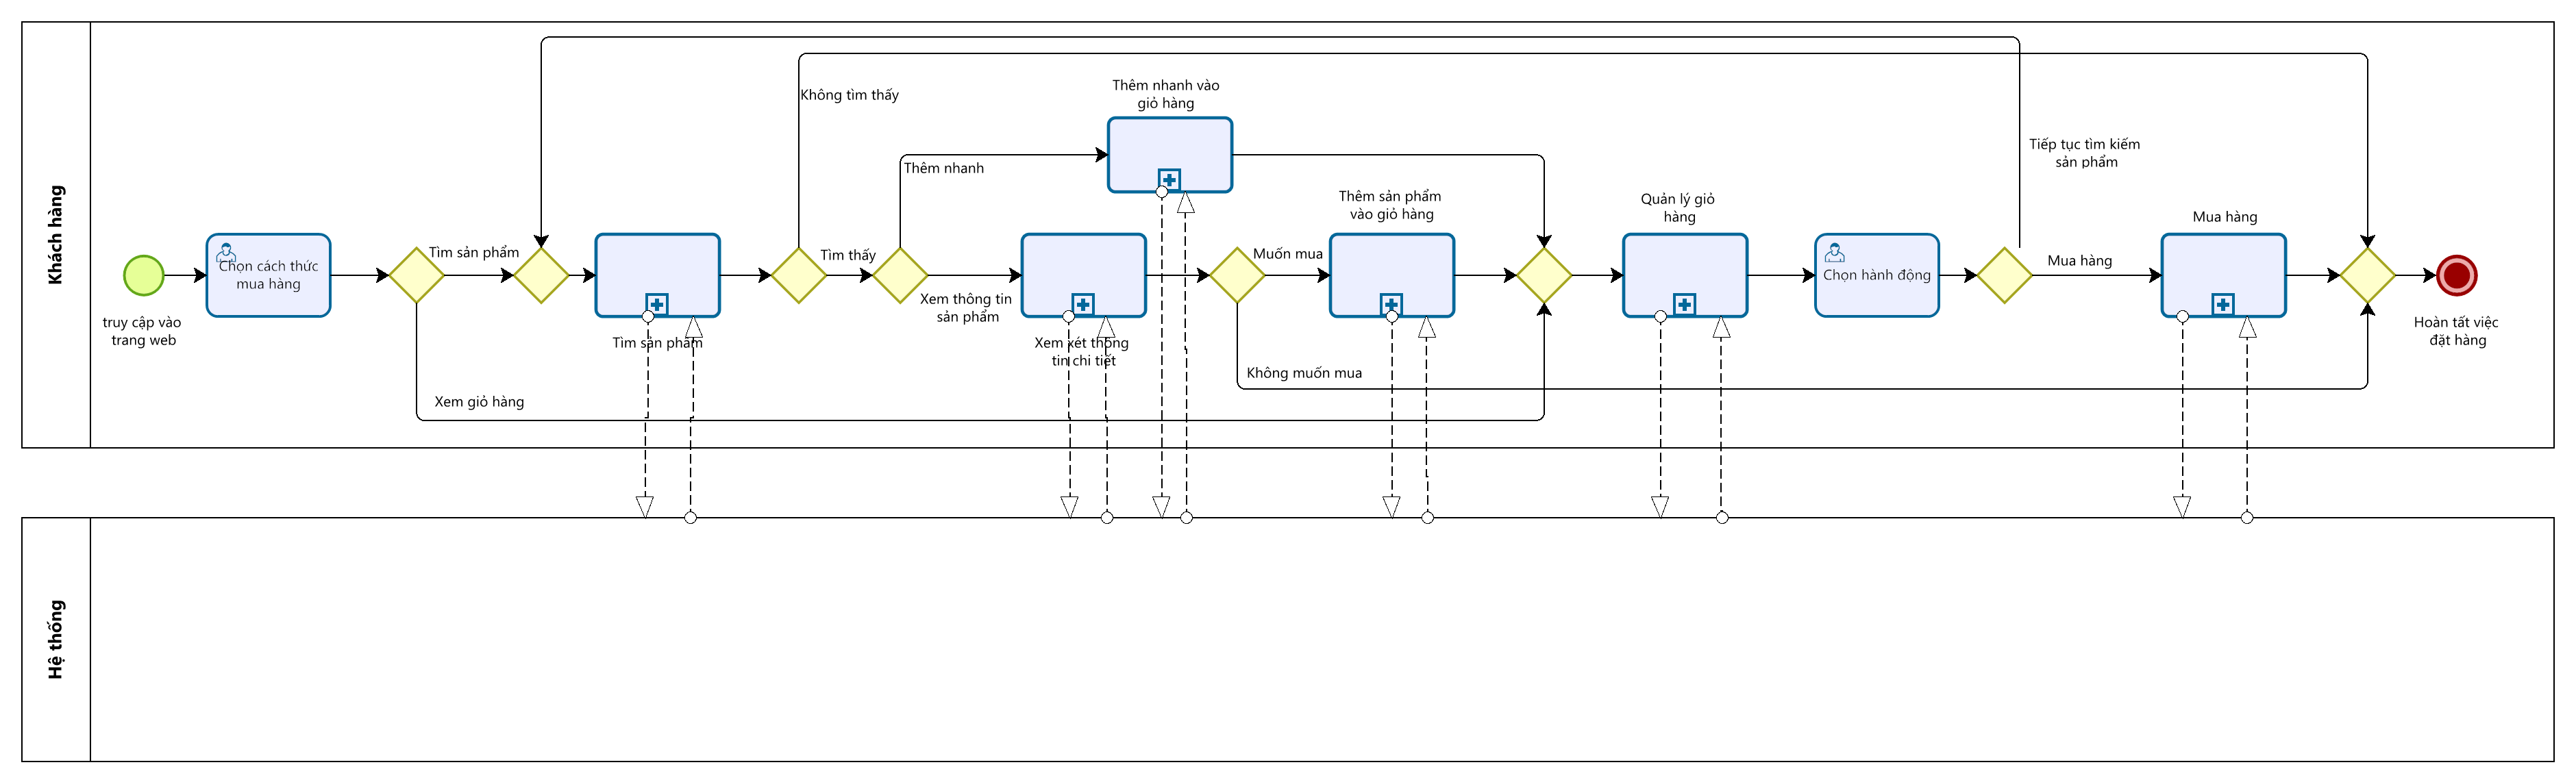
\includegraphics[width=17cm]{img/BPMN/customer_buy/customer_buy.png}
        \newline
        \caption{Lược đồ BPMN cho quy trình khách hàng mua hàng}
    \end{figure}
    \textbf{Mô tả:} Quy trình bắt đầu khi người dùng bắt đầu truy cập vào trang web, khách hàng chọn cách thức mua hàng là bắt đầu từ tìm sản phẩm hoặc là bắt đầu mua từ những sản phẩm đã có sẵn trong giỏ hàng. Khi người dùng chọn tìm sản phẩm thì người dùng sẽ thực hiện quy trình con (sub-process) "Tìm sản phẩm". Sau khi thực hiện xong tìm sản phẩm và tìm thấy thì người dùng thực hiện xem thông tin chi tiết để hiểu rõ hơn về sản phẩm và quyết định có muốn thêm sản phẩm vào giỏ hàng hay không; hoặc khi người dùng đã biết về sản phẩm thì có thể thêm chọn thêm nhanh sản phẩm vào giỏ hàng. Sau khi thêm sản phẩm vào giỏ hàng thì người dùng thực hiện quy trình con quản lý giỏ hàng để lựa chọn cũng như cập nhật các đặc điểm mà người dùng mong muốn ở sản phẩm. Sau khi quản lý xong giỏ hàng thì người dùng cần chọn hành động tiếp tục tìm kiếm thêm sản phẩm để mua hàng hoặc là trực tiếp đi đến quy trình con "Mua hàng" và sau đó là kết thúc quy trình.


    \begin{figure}[!htp]
        \centering
        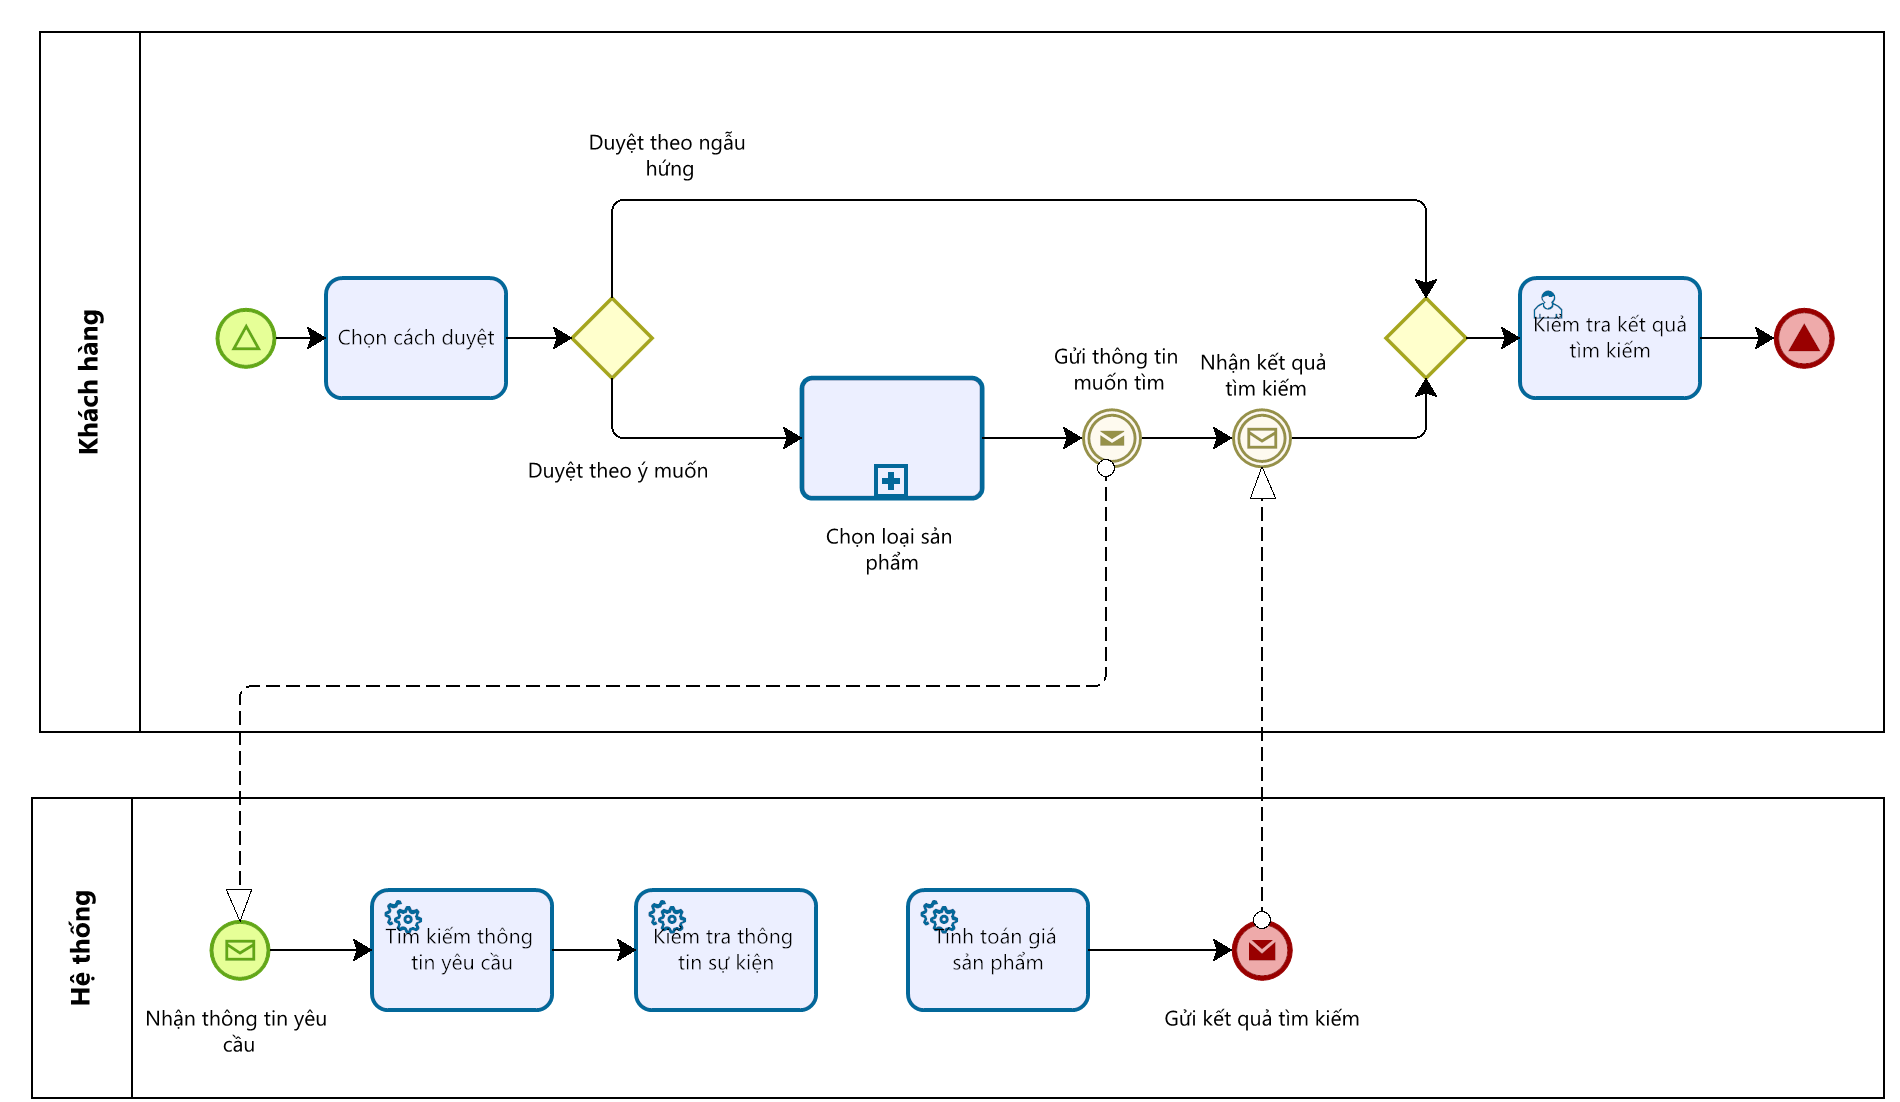
\includegraphics[width=13cm]{img/BPMN/customer_buy/customer_search_product.png}
        \newline
        \caption{Lược đồ BPMN cho quy trình con tìm kiếm sản phẩm}
    \end{figure}
    \textbf{Mô tả:} Đây là 1 quy trình con chứa quy trình tìm kiếm sản phẩm mà người dùng muốn tìm kiếm. Bắt đầu từ việc chọn cách duyệt bằng cách duyệt theo ngẫu hứng hay duyệt theo ý muốn. Khi người dũng duyệt theo ý muốn thì thực hiện quy trình con "Chọn loại sản phẩm" để chọn nhưng loại sản phẩm theo ý muốn của khách hàng. Sau khi chọn loại sản phẩm thì hệ thống sẽ nhận thông tin và xử lý, sau đó phản hồi kết quả và người dùng kiểm tra kết quả tìm kiếm và kết thúc quy trình con này.

    \begin{figure}[!htp]
        \centering
        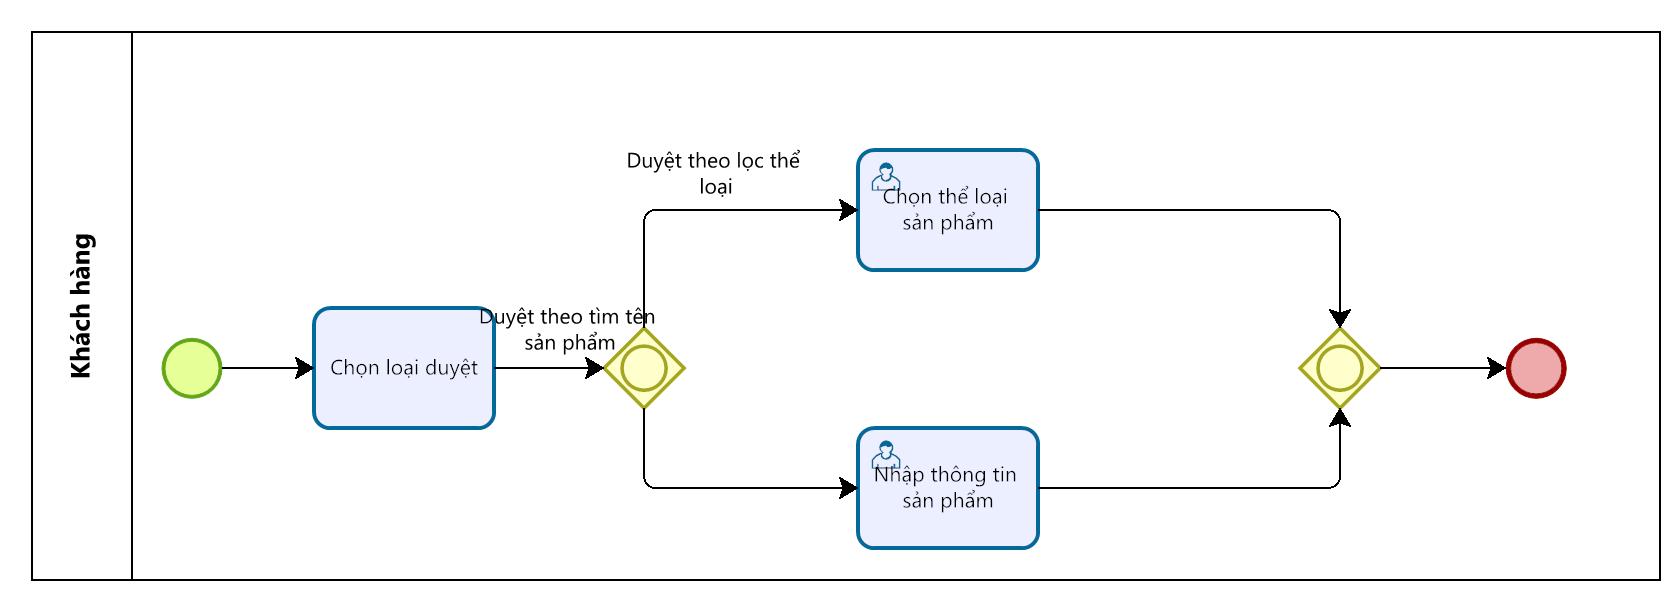
\includegraphics[width=12cm]{img/BPMN/customer_buy/customer_select_type.png}
        \newline
        \caption{Lược đồ BPMN cho quy trình con chọn loại sản phẩm mà khác hàng muốn tìm}
    \end{figure}
    \textbf{Mô tả:} Đây là 1 quy trình con chứa quy trình chọn loại sản phẩm mà người dùng muốn tìm kiếm. Bắt đầu từ việc chọn loại duyệt thì người dùng có thể chọn duyệt theo thể loại hoặc duyệt theo tên tìm kiếm hoặc duyệt theo sự kiện.
    
    \begin{figure}[!htp]
        \centering
        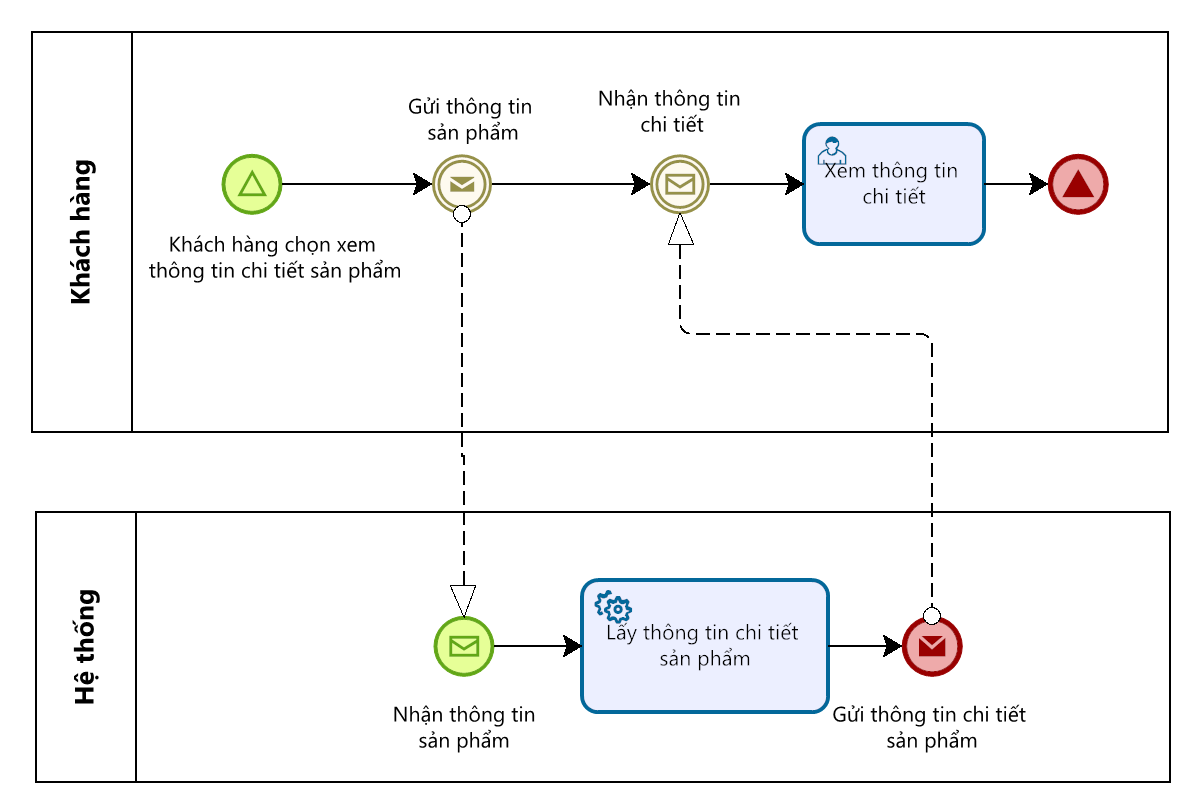
\includegraphics[width=12cm]{img/BPMN/customer_buy/customer_product_detail.png}
        \newline
        \caption{Lược đồ BPMN cho quy trình xem xét thông tin chi tiết của sản phẩm}
    \end{figure}
    \textbf{Mô tả:} Đây là 1 quy trình con chứa quy trình xem thông tin chi tiết của sản phẩm, sau khi khách hàng chọn sản phẩm muốn xem thông tin chi tiết thì hệ thống sẽ thực hiện lấy thông tin chi tiết sản phẩm từ cơ sở dữ liệu và phản hồi kết quả về cho khách hàng. Sau khi nhận được kết quả thì khách hàng xem thông tin chi tiết của sản phẩm và kết thúc quy trình.

    \begin{figure}[!htp]
        \centering
        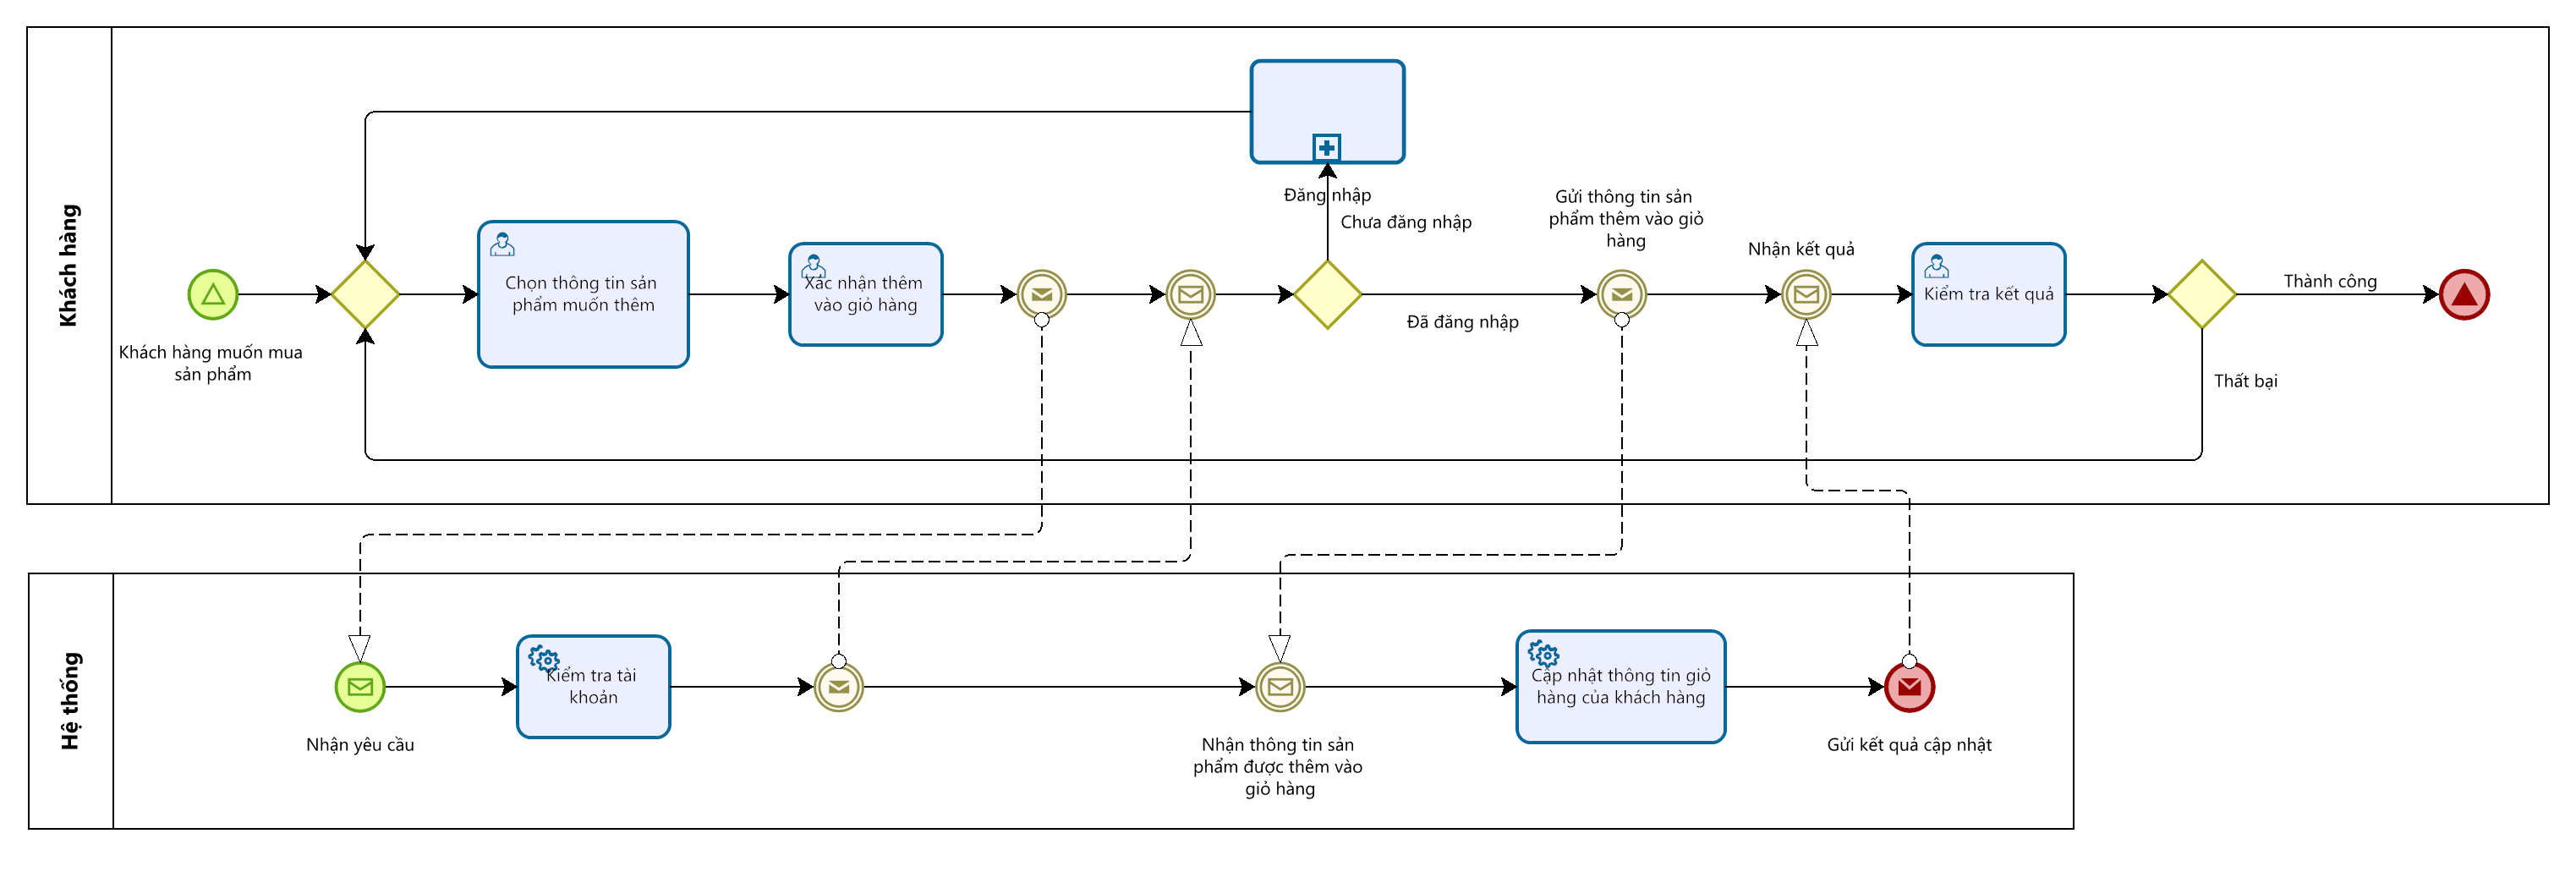
\includegraphics[width=15cm]{img/BPMN/customer_buy/customer_add_to_card.png}
        \newline
        \caption{Lược đồ BPMN cho quy trình thêm sản phẩm vào giỏ hàng}
    \end{figure} 
    \textbf{Mô tả:} Đây là 1 quy trình con chứa quy trình thêm sản phẩm vào giỏ hàng, sau khi khách hàng xem thông tin chi tiết và muốn mua sản phẩm thì người dùng các thông tin sản phẩm mà khách hàng muốn thêm sau đó xác nhận thêm vào giỏ hàng. Thông tin sản phẩm khách hàng chọn thêm vào giỏ hàng được gửi đi và hệ thống thực hiện kiểm tra tài khoản khách hàng đã đăng nhập chưa, sau khi xác nhận được đã đăng nhập thì hệ thống kiểm tra thông tin và cập nhật thông tin sản phẩm vào giỏ hàng, sau đó gửi kết quả về phía khách hàng. Sau khi nhận được kết quả thì người dùng kiểm tra kết quả và kết thúc quy trình.
     
    \begin{figure}[!htp]
        \centering
        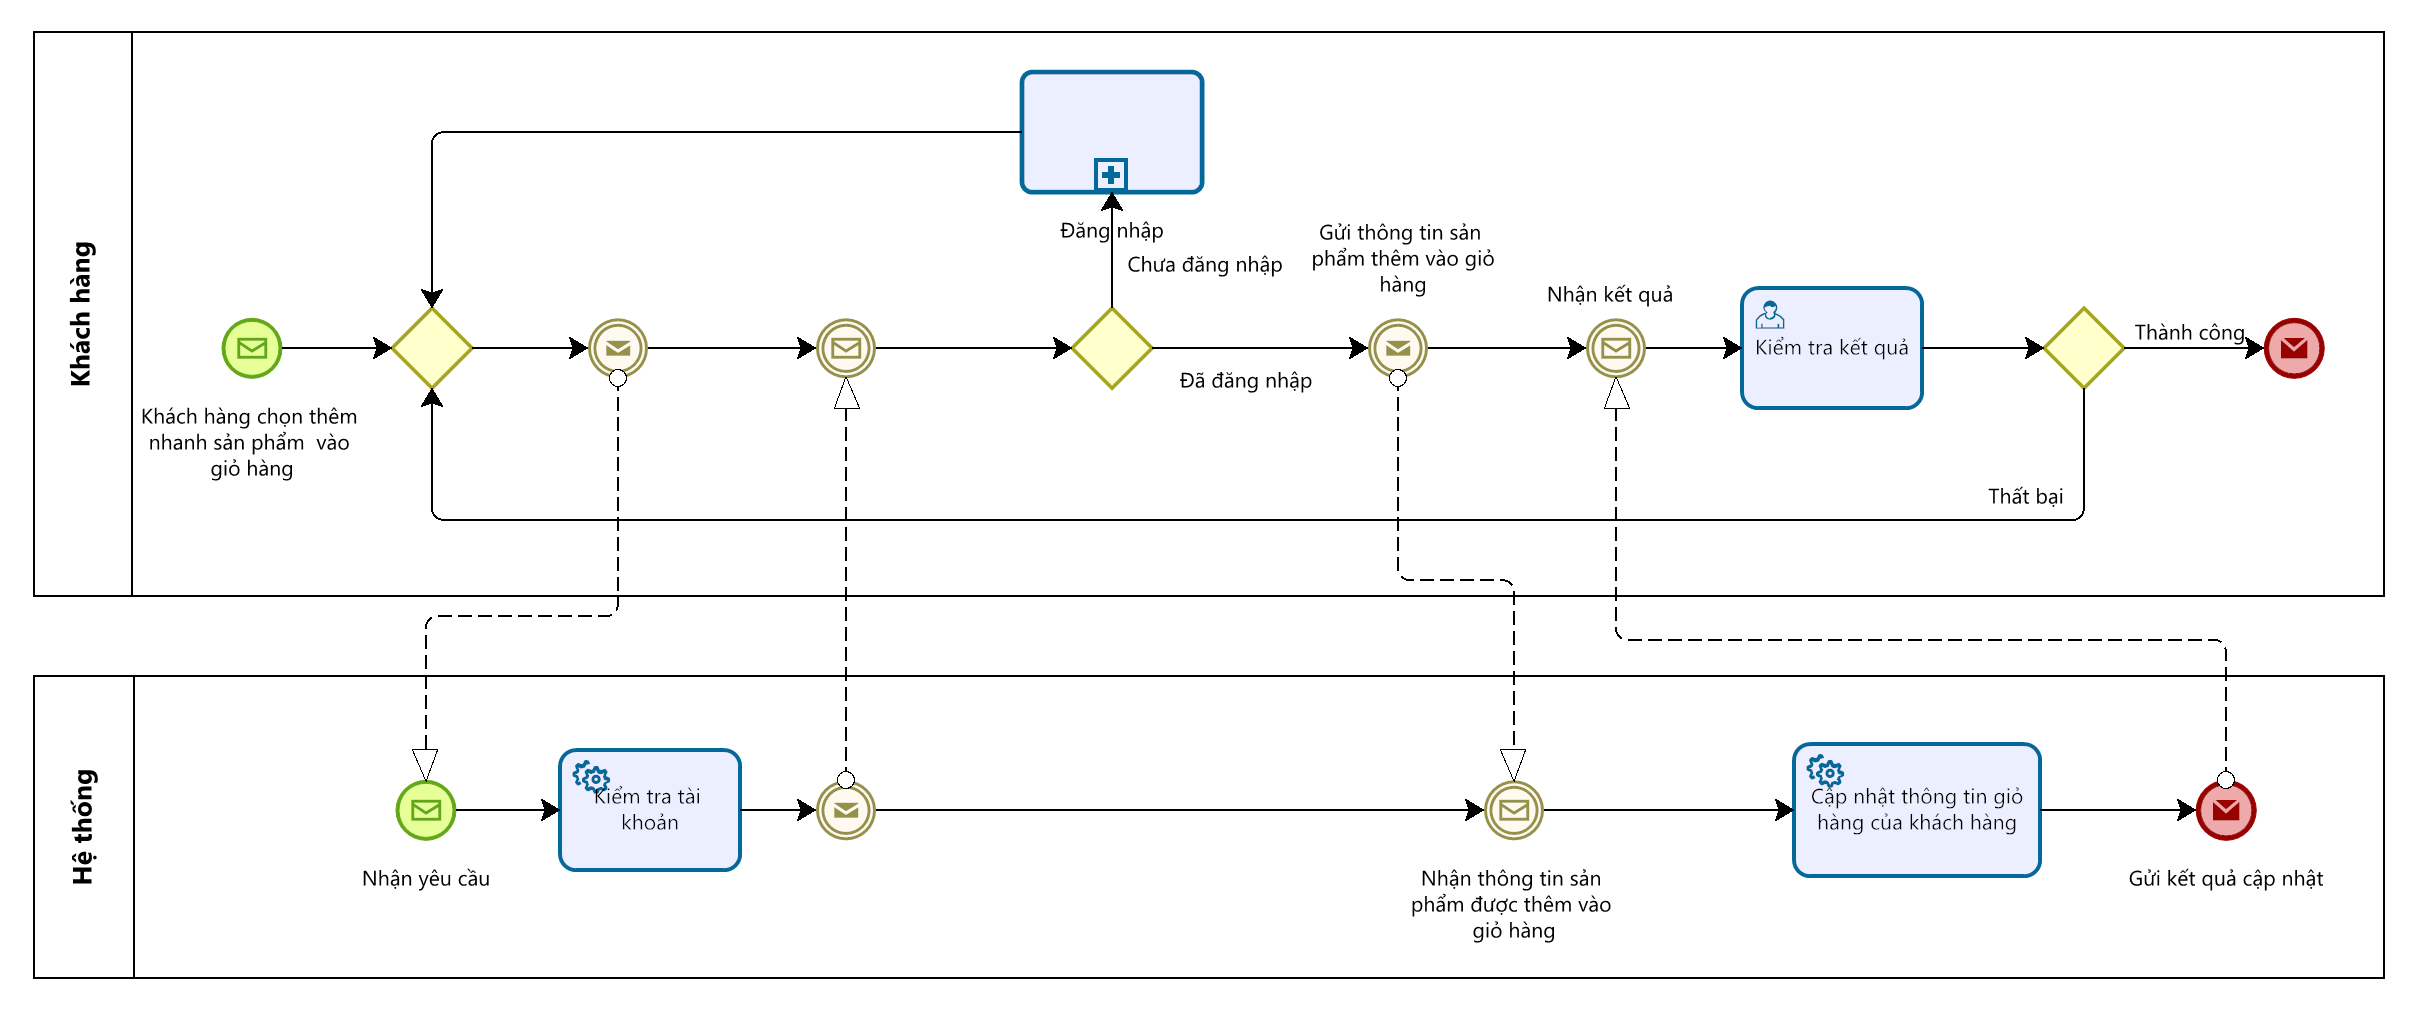
\includegraphics[width=15cm]{img/BPMN/customer_buy/customer_add_fast.png}
        \newline
        \caption{Lược đồ BPMN cho quy trình thêm nhanh sản phẩm vào giỏ hàng}
    \end{figure}
    \textbf{Mô tả:} Đây là 1 quy trình con chứa quy trình thêm nhanh sản phẩm vào giỏ hàng, sau khi khách hàng chọn thêm nhanh sản phẩm vào giỏ hàng. Thông tin sản phẩm khách hàng chọn thêm vào giỏ hàng được gửi đi và hệ thống thực hiện kiểm tra tài khoản khách hàng đã đăng nhập chưa, sau khi xác nhận được đã đăng nhập thì hệ thống kiểm tra thông tin và cập nhật thông tin sản phẩm vào giỏ hàng, sau đó gửi kết quả về phía khách hàng. Sau khi nhận được kết quả thì người dùng kiểm tra kết quả và kết thúc quy trình.
 
    \begin{figure}[!htp]
        \centering
        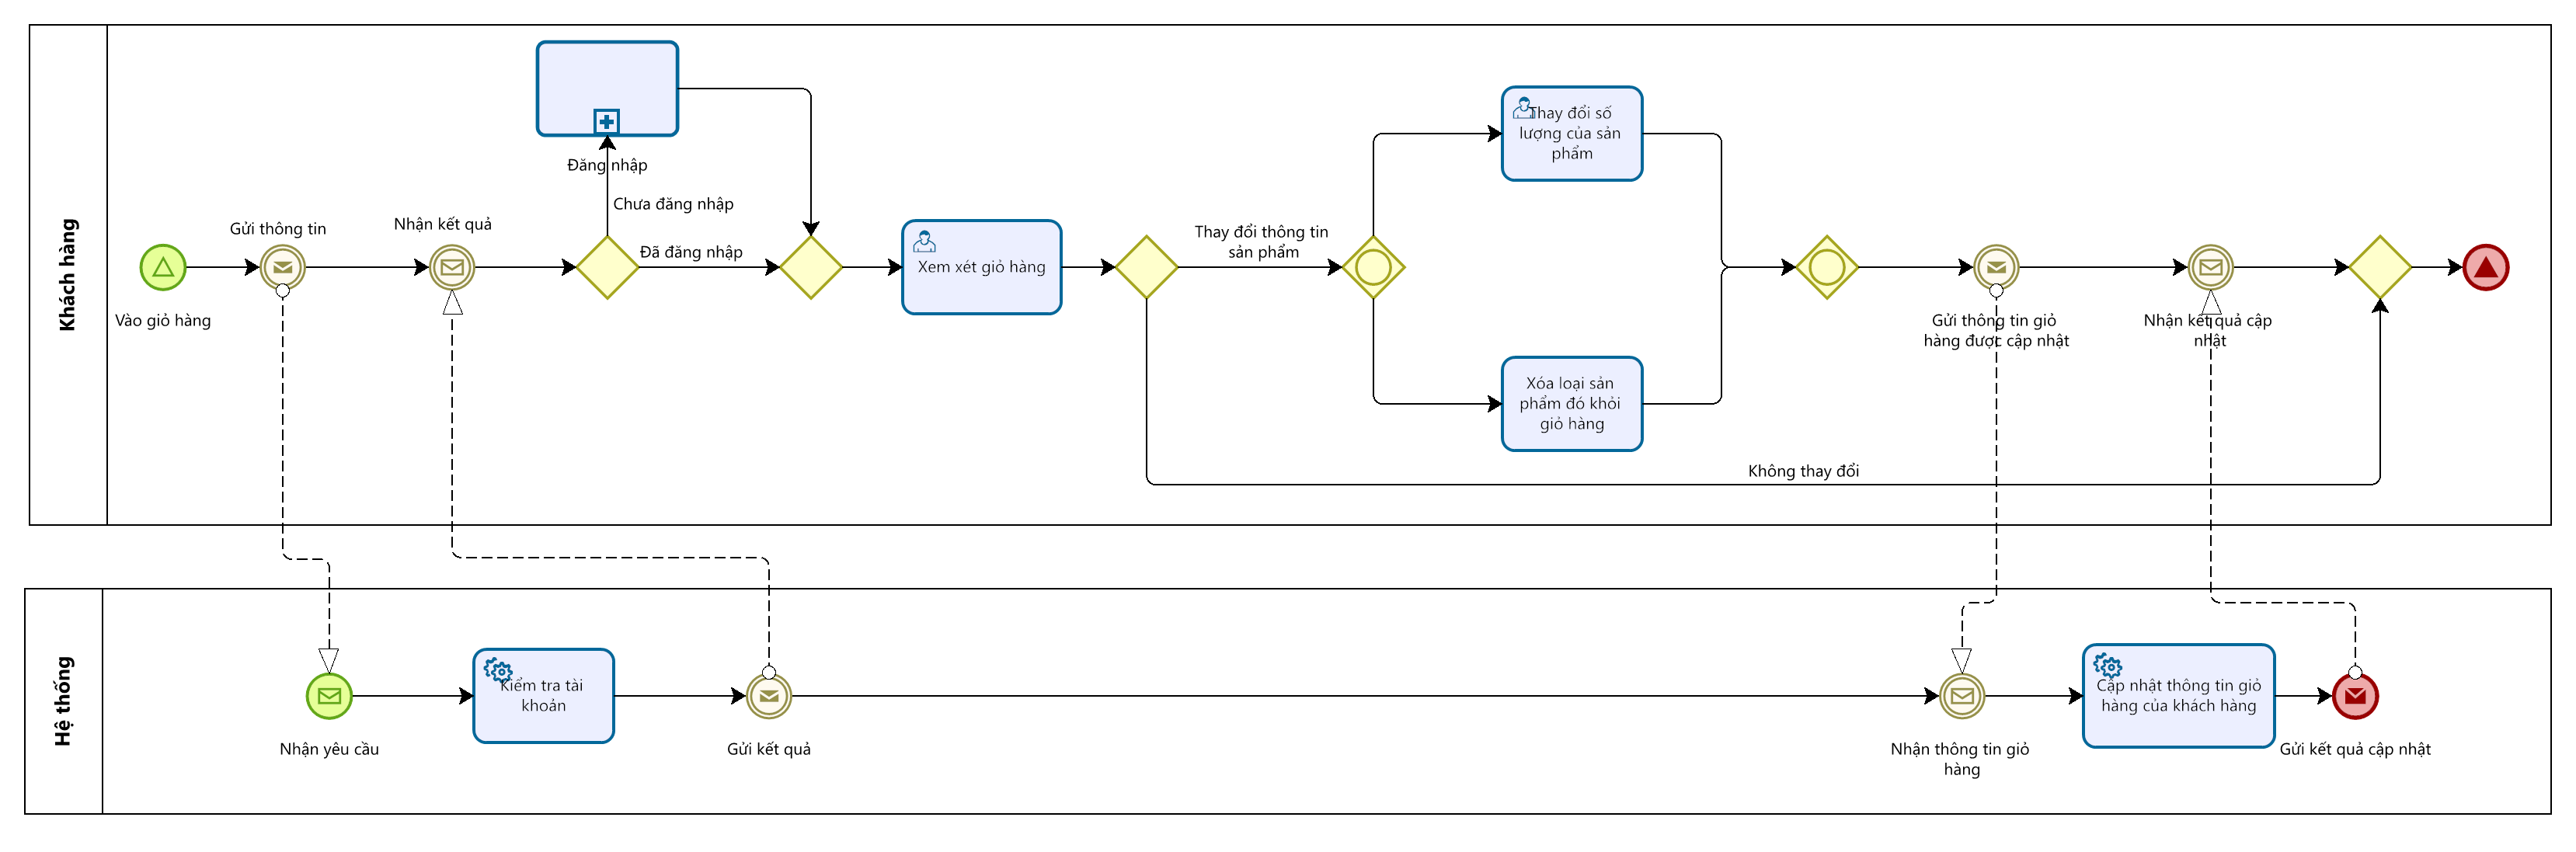
\includegraphics[width=15cm]{img/BPMN/customer_buy/customer_cart.png}
        \newline
        \caption{Lược đồ BPMN cho quy trình quản lý giỏ hàng}
    \end{figure}
    \textbf{Mô tả:} Đây là 1 quy trình con chứa quy trình quản lý giỏ hàng. Quy trình bắt đầu từ khi khách hàng chọn vào giỏ hàng. Hệ thống thực hiện kiểm tra tài khoản rồi sau đó truy xuất dữ liệu giỏ hàng của tài khoản khách hàng và phản hồi về lại cho khách hàng. Khách hàng thực thực hiện xem xét giỏ hàng và thực hiện thay đổi thông tin sản phẩm trong giỏ hàng bằng cách thay đổi thông tin sản phẩm hay xóa sản phẩm khỏi giỏ hàng, hệ thống nhận thông tin thay đổi sau đó kiểm tra thông tin và cập nhật thông tin giỏ hàng rồi trả về kết quả, khách hàng nhận kết quả và kết thúc quy trình.
 
    \begin{figure}[!htp]
        \centering
        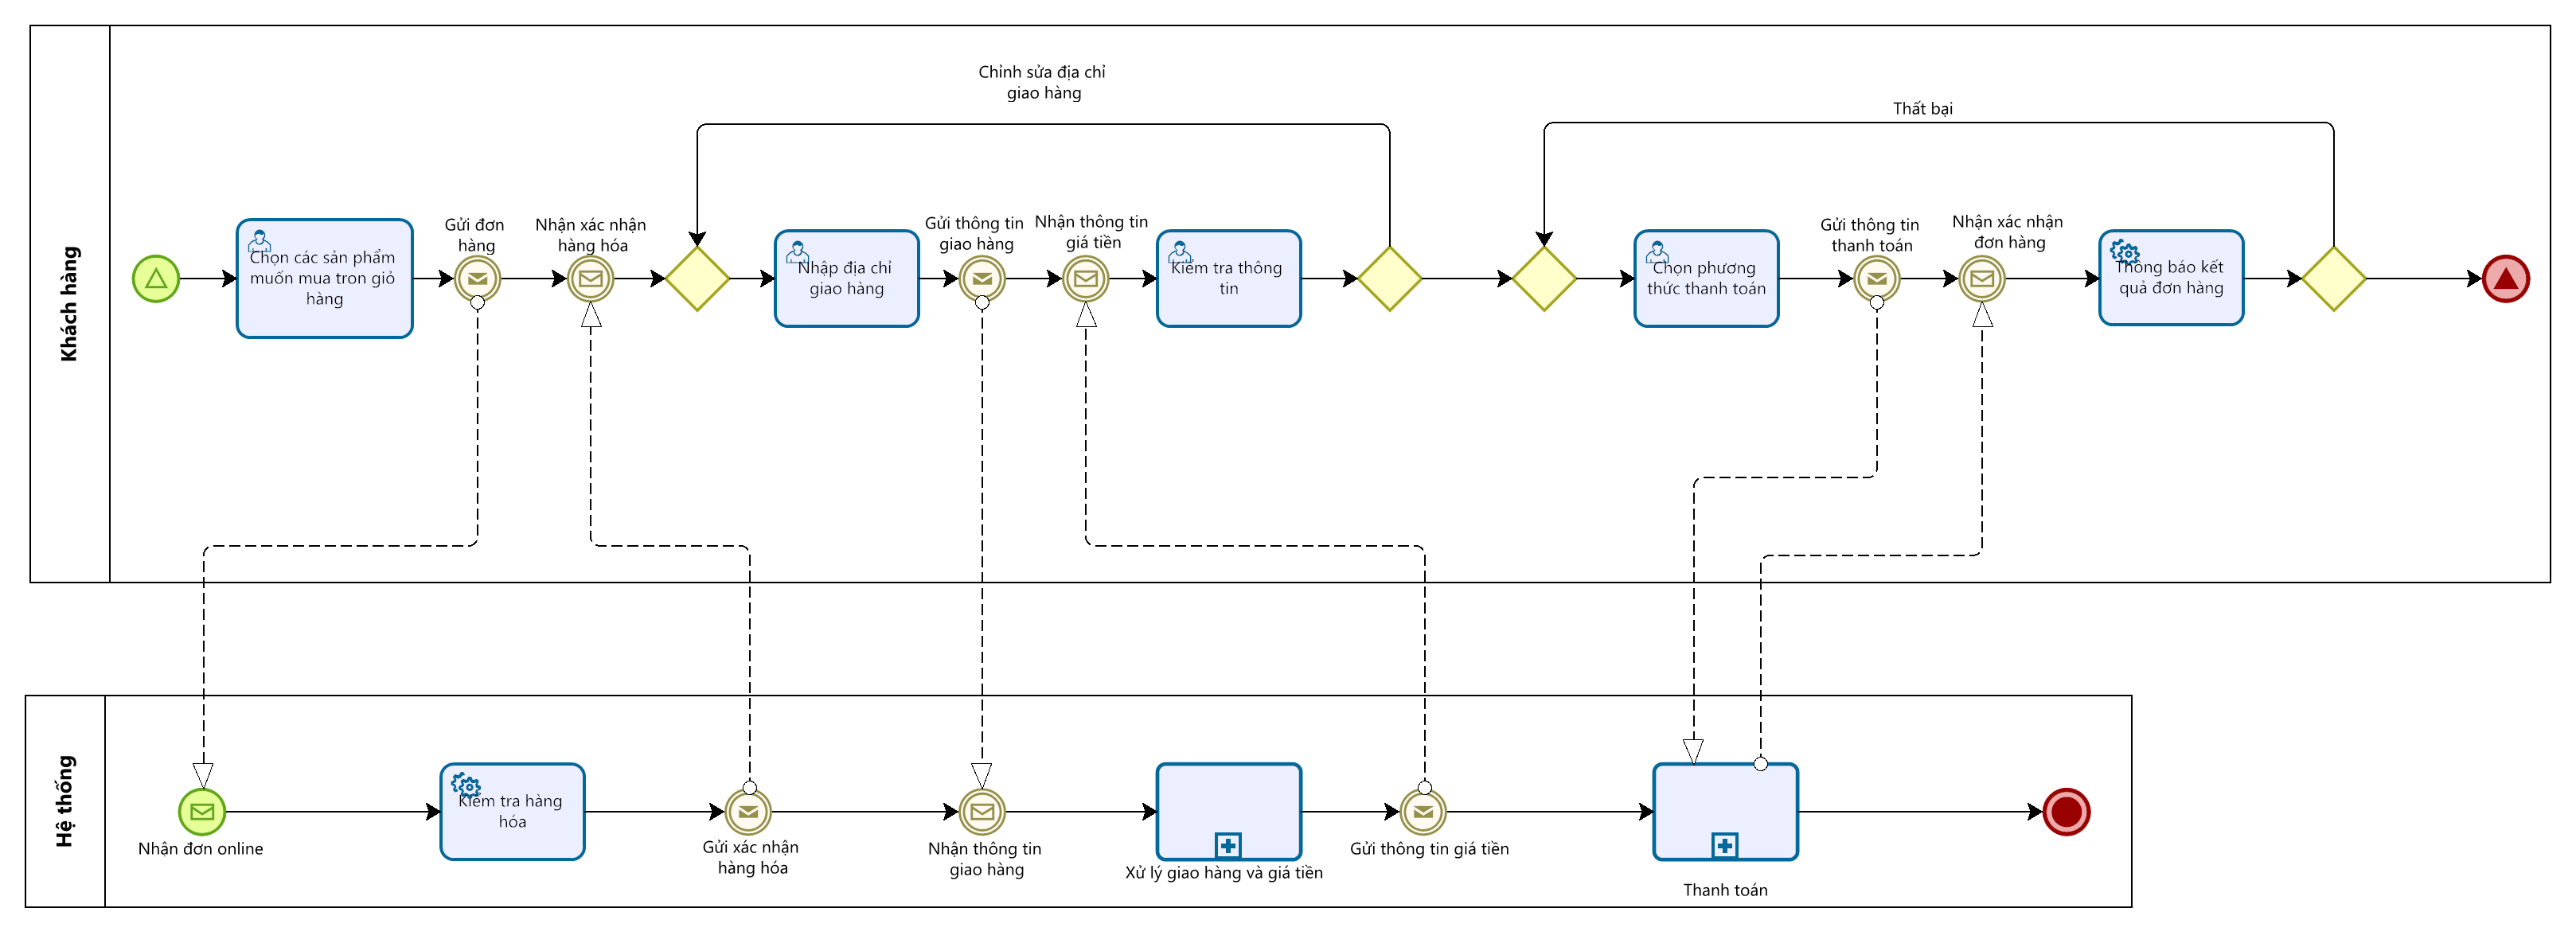
\includegraphics[width=15cm]{img/BPMN/customer_buy/customer_buy_order.png}
        \newline
        \caption{Lược đồ BPMN cho quy trình mua hàng}
    \end{figure}
    \textbf{Mô tả:} Đây là 1 quy trình con chứa quy trình đặt mua hàng của khách hàng. Khách hàng chọn các sản phẩm trong giỏ hàng mà bản thân muốn mua và chọn "Đặt hàng". Hệ thống thực hiện kiểm tra hàng hóa và phản hồi về lại cho khách hàng. Sau khi chọn "Đặt hàng" và nhận kết quả xác nhận hàng hóa, khách hàng thực thực hiện nhập địa chỉ giao hàng, hệ thống sẽ thực hiện xử lý giao hàng và giá tiền để tính tổng hóa hơn cho khách hàng. Khách hàng thực hiện kiểm tra thông tin sau khi nhận lại thông tin giá tiền, nếu chưa chính xác về địa chỉ gia hàng thì quay lại nhập địa chỉ giao hàng, nếu đã chính xác thì thực hiện chọn phương thức thanh toán và chọn "Thanh toán". Hệ thống kiểm tra thông tin thanh toán mà người dùng chọn sau đó thực hiện quy trình "Thanh toán", sau khi kết thúc quy trình thanh toán thì hệ thống phản hồi và hiển thị thông báo kết quả đơn hàng, nếu thành công thì kết thúc quy trình, nếu thất bại thì khách hàng quay lại chọn phương thức thanh toán phù hợp.
 
    \begin{figure}[!htp]
        \centering
        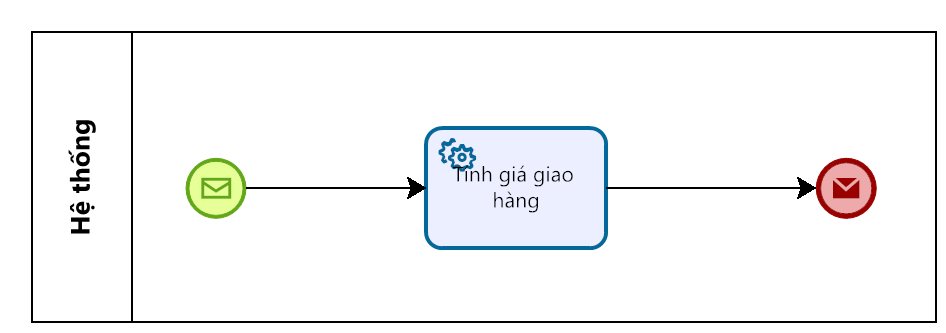
\includegraphics[width=5in]{img/BPMN/customer_buy/customer_calc_fee.png}
        \newline
        \caption{Lược đồ BPMN cho quy trình tính toán chi phí đơn hàng}
    \end{figure}
    \textbf{Mô tả:} Đây là 1 quy trình con chứa quy trình tính toán chi phí đơn hàng. Hệ thống thực hiện kiểm tra kho để tạo đơn hàng vận chuyển, nếu không có kho nào đủ hàng cho khách hàng thì cần thực hiện tính toán trao đổi kho và gửi thông tin trao đổi hàng cho kho. Sau khi thực hiện tính toán kho thì thực hiện tính toán giá giao hàng và tính tổng tiền của đơn hàng.
 
    \begin{figure}[!htp]
        \centering
        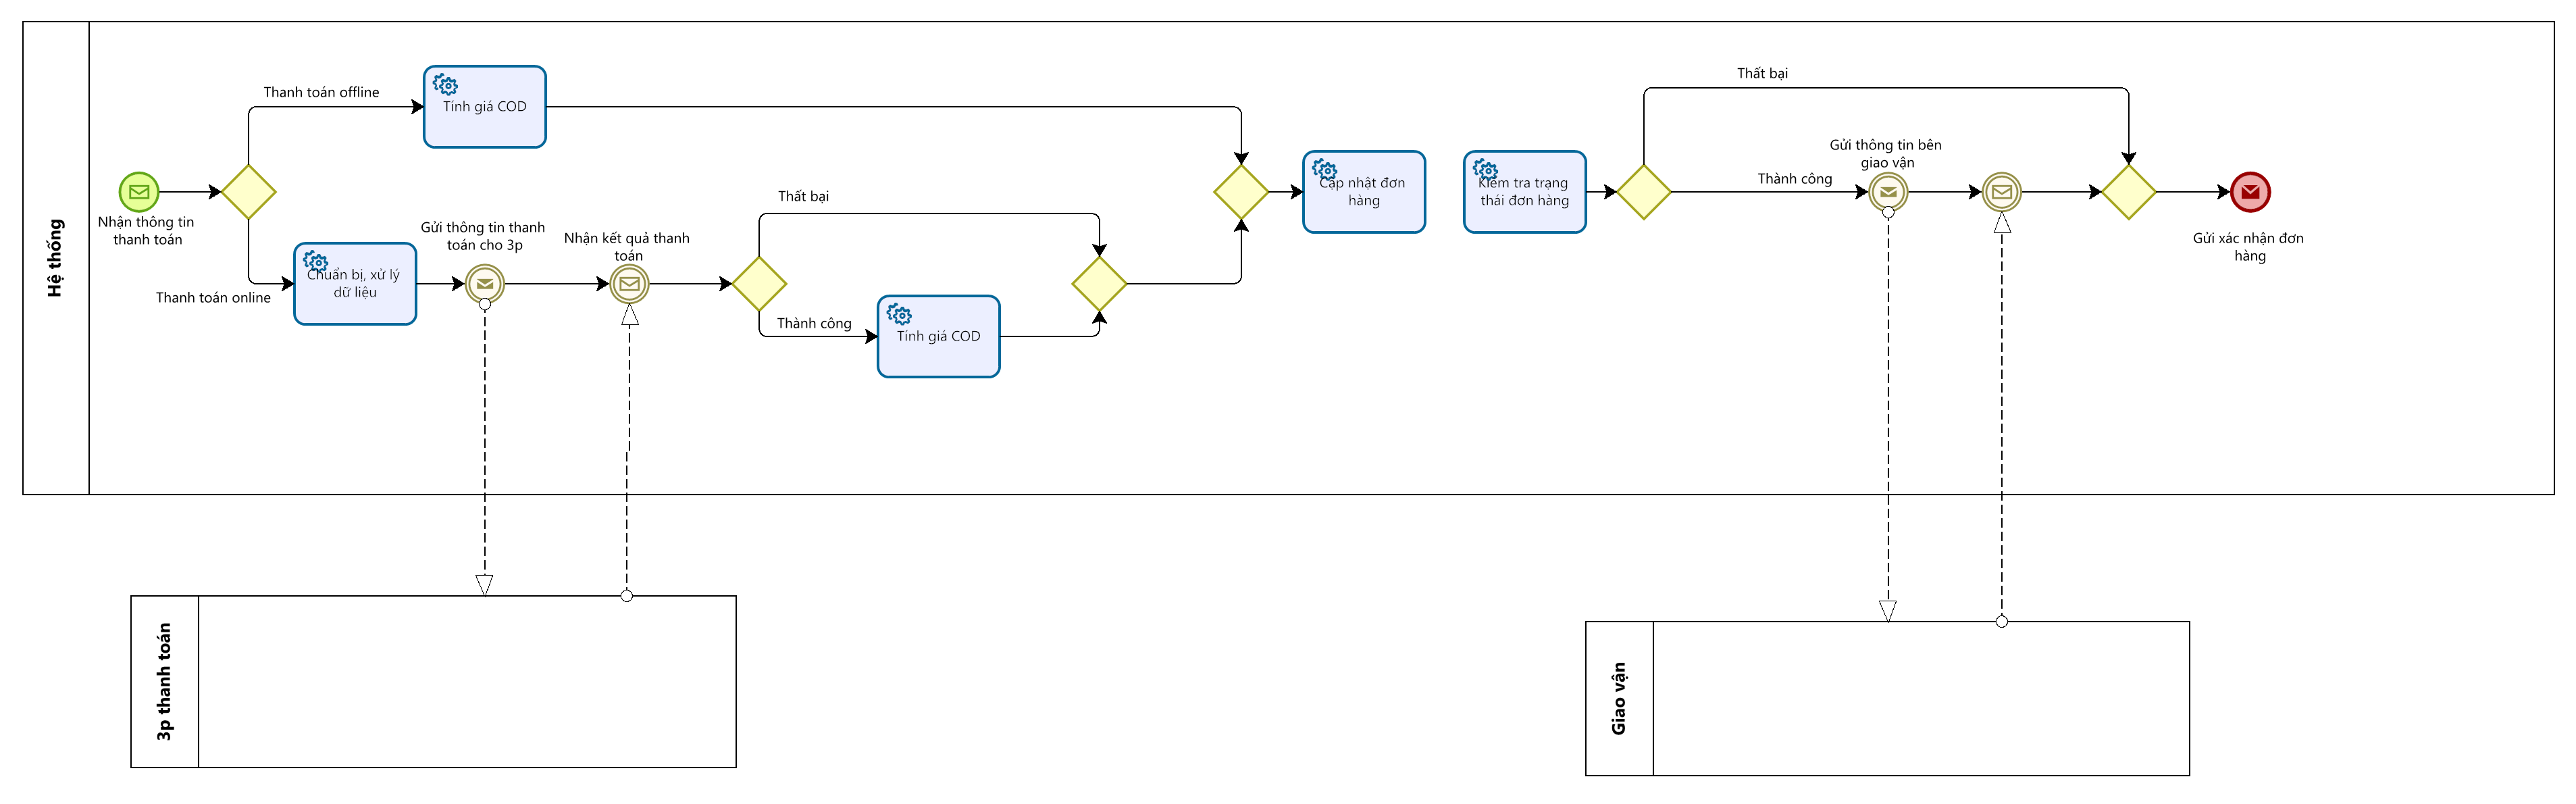
\includegraphics[width=15cm]{img/BPMN/customer_buy/customer_payment.png}
        \newline
        \caption{Lược đồ BPMN cho quy trình thanh toán đơn hàng}
    \end{figure}
    \textbf{Mô tả:} Đây là 1 quy trình con chứa quy trình thanh toán đơn hàng. Quy trình bắt đầu từ sự kiện nhận thông tin thanh toán, nếu thanh toán trực tiếp khi nhận hàng thì thực hiện cập nhật đơn hàng. Nếu phương thức thanh toán là trực tuyên thì hệ thống thực hiện gửi thông tin thanh toán cho bên thứ ba tương ứng với bên mà người dùng chọn, sau đó chờ bên thứ ba trả về kết quả thanh toán. Sau khi nhận được kết quả từ bên thứ ba thì thông báo kết quả với người dùng, nếu thanh toán thành công thì thực hiện cập nhật đơn hàng vào hệ thống, khi cập nhật đơn hàng thành công thì thực hiện gửi thông tin vận chuyển đến dịch vụ vận chuyển của bên thứ ba và kết thúc quy trình.
 

\newpage
\subsection{Quản lý sự kiện}

\subsubsection{Thêm sự kiện}

\begin{figure}[!htp]
    \centering
    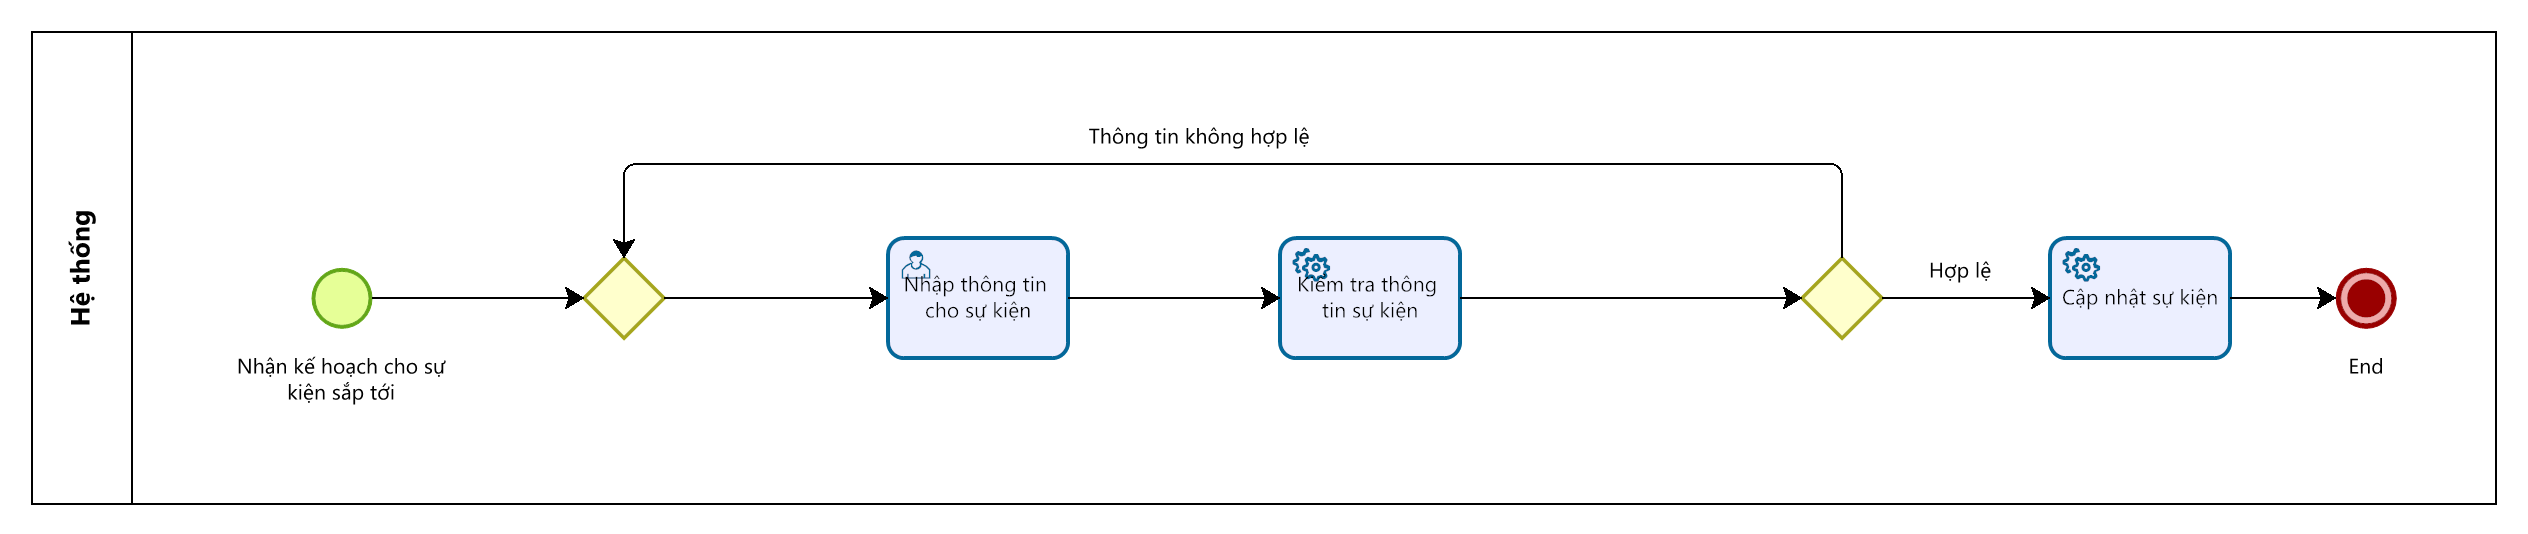
\includegraphics[width=14cm]{img/BPMN/event/add_event.png}
    \newline
    \caption{Lược đồ BPMN cho quy trình thêm sự kiện}
\end{figure}
Mô tả: quy trình được bắt đầu bởi sự kiện nhận thông tin cho sự kiện sắp tới, sau khi nhận được thông tin sự kiện mới thì quản trị viên nhập thông tin cho sự kiện và xác nhận tạo sự kiện. Sau khi thông tin sự kiện mới được gửi đi thì hệ thống sẽ kiểm tra thông tin sự kiện có hợp lệ hay không, nếu hợp lệ thì cập nhật sự kiện mới vào hệ thống và kết thúc quy trình, nếu không hợp lệ thì quản trị viên cần quay lại task nhập lại thông tin cho sự kiện.

\subsubsection{Sửa sự kiện}

\begin{figure}[!htp]
    \centering
    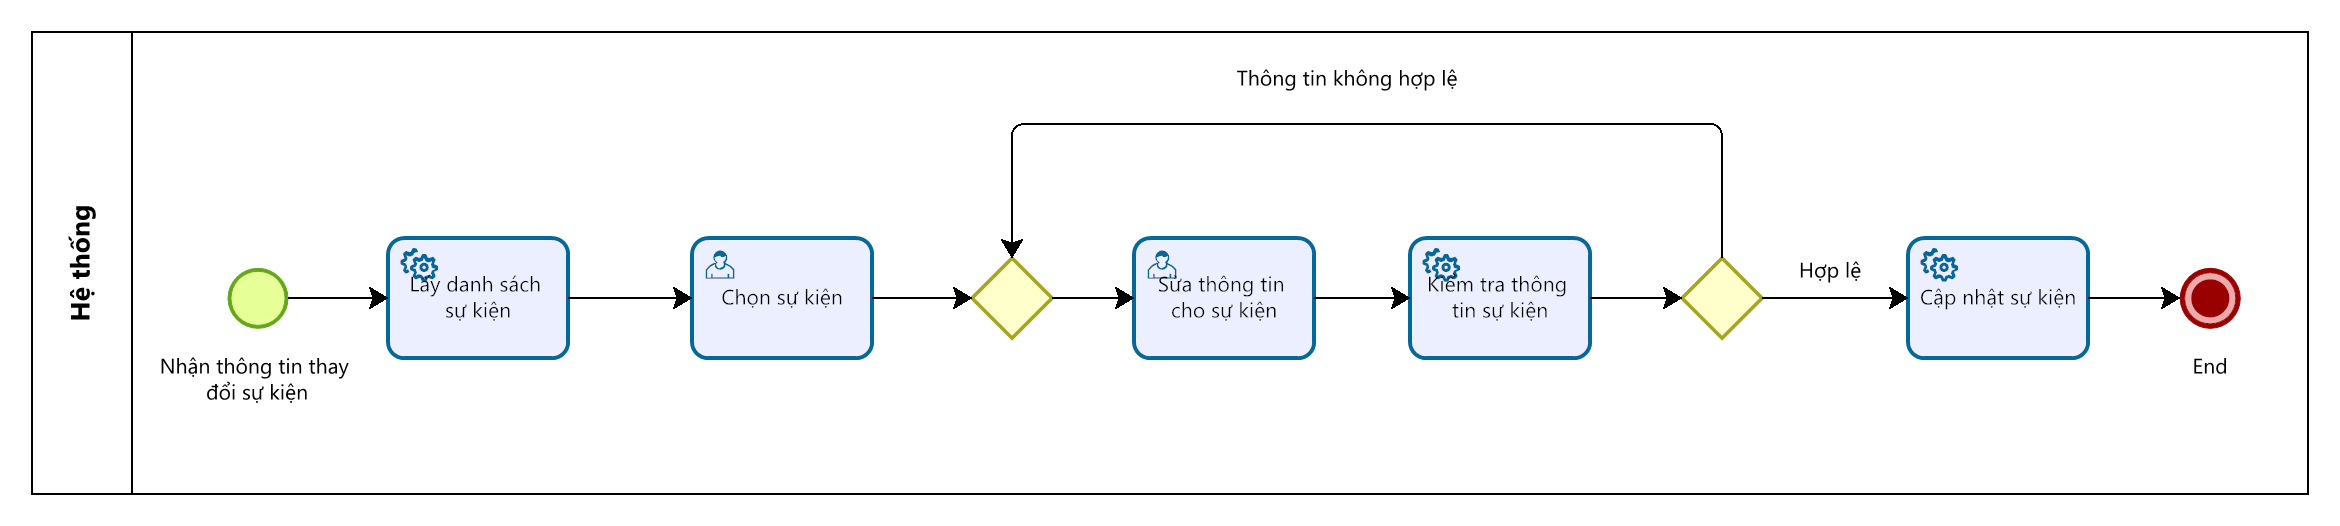
\includegraphics[width=14cm]{img/BPMN/event/edit_event.png}
    \newline
    \caption{Lược đồ BPMN cho quy trình chỉnh sửa sự kiện}
\end{figure}
Mô tả: quy trình được bắt đầu bởi sự kiện nhận thông tin thay đổi sự kiện, sau khi nhận được thông tin sự kiện cần cập nhật thì quản trị viên chọn sự cần cần sửa, sau đó nhập thông tin cho sự kiện và xác nhận cập nhật sự kiện. Sau khi thông tin cập nhật sự kiện được gửi đi thì hệ thống sẽ kiểm tra thông tin sự kiện có hợp lệ hay không, nếu hợp lệ thì cập nhật lại sự kiện vào hệ thống và kết thúc quy trình, nếu không hợp lệ thì quản trị viên cần quay lại task nhập lại thông tin cho sự kiện.

\subsubsection{Xóa sự kiện}

\begin{figure}[!htp]
    \centering
    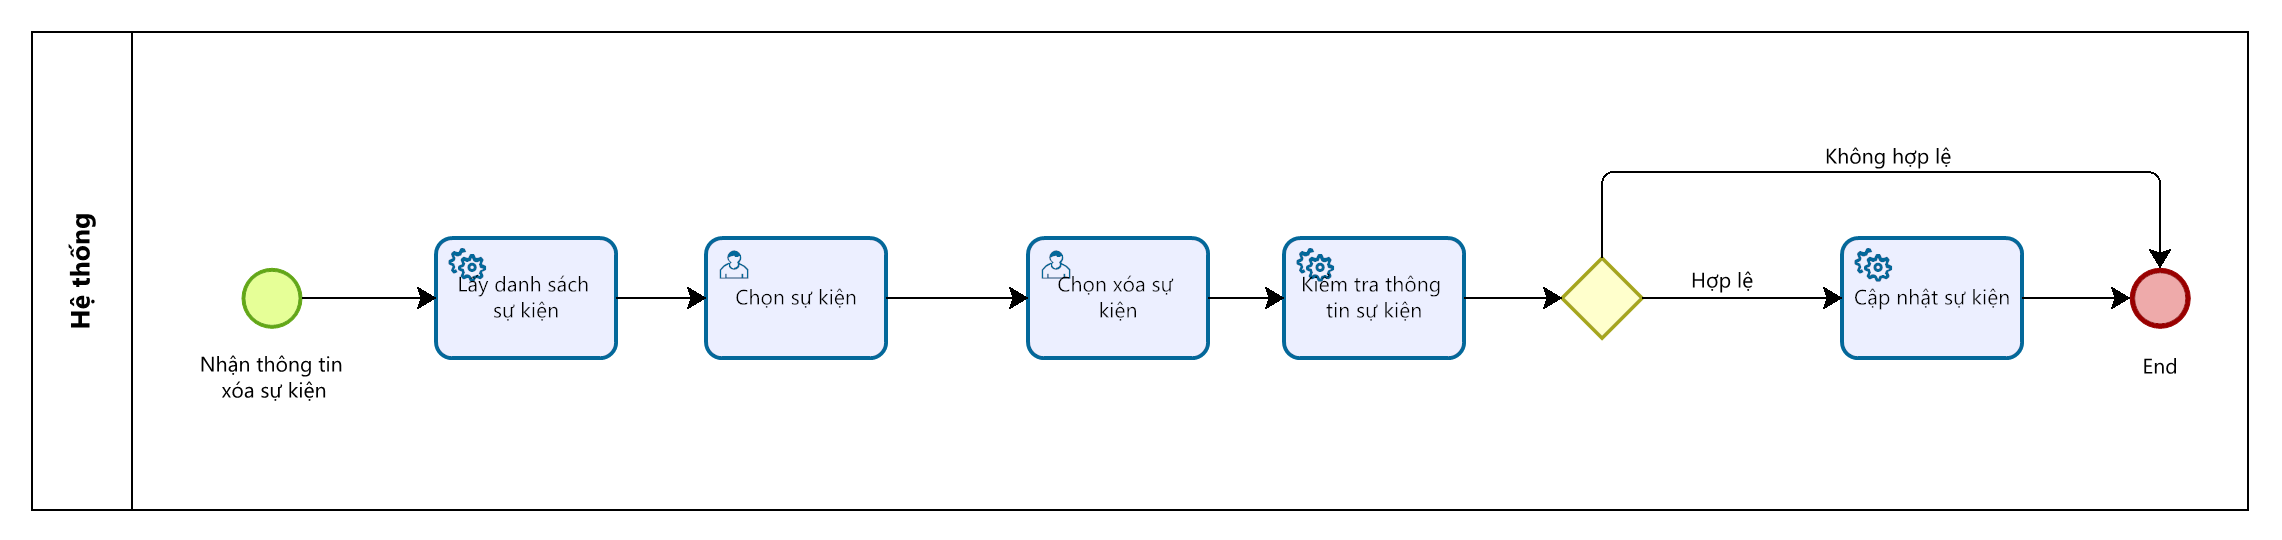
\includegraphics[width=14cm]{img/BPMN/event/delete_event.png}
    \newline
    \caption{Lược đồ BPMN cho quy trình xóa sự kiện}
\end{figure}
Mô tả: quy trình được bắt đầu bởi sự kiện nhận thông tin xóa sự kiện, sau khi nhận được thông tin sự kiện cần cập nhật thì quản trị viên chọn sự cần cần xóa và chọn xóa sự kiện. Sau khi thông tin sự kiện cần xóa được gửi đi thì hệ thống sẽ kiểm tra thông tin sự kiện có hợp lệ hay không, nếu hợp lệ thì cập nhật xóa sự kiện khỏi hệ thống và kết thúc quy trình, nếu không hợp lệ thì thông báo thất bại và kết thúc quy trình.

\subsection{Khách hàng mua hàng trực tiếp}
\begin{figure}[!htp]
    \centering
    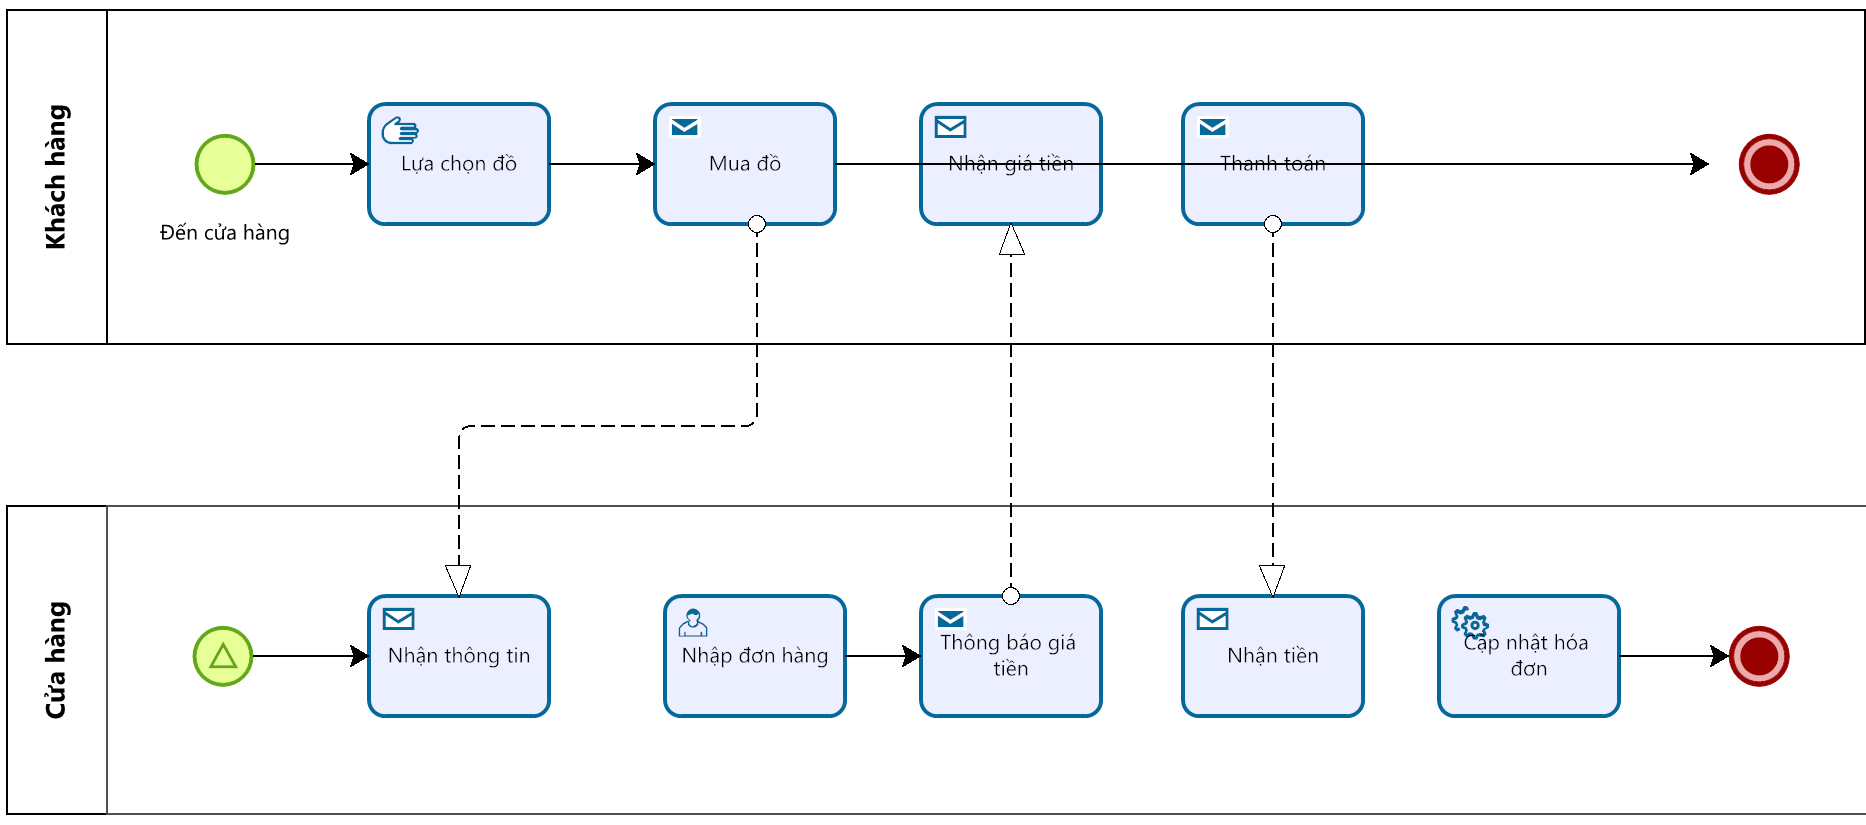
\includegraphics[width=14cm]{img/BPMN/Hien/Customer_buyOffline.png}
    \newline
    \caption{Lược đồ BPMN cho quy trình khách hàng mua hàng trực tiếp}
\end{figure}

\subsection{Đăng nhập}
\begin{figure}[!htp]
    \centering
    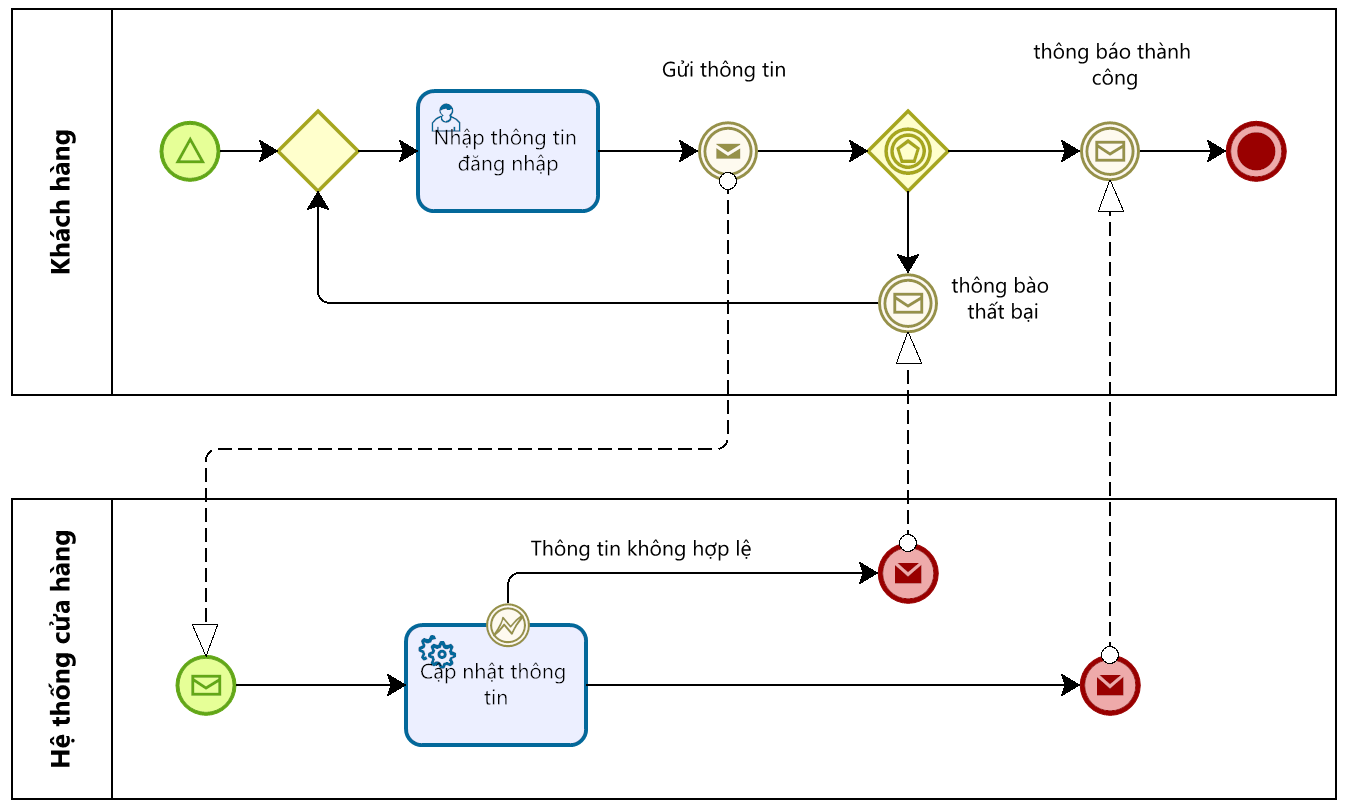
\includegraphics[width=14cm]{img/BPMN/Hien/Customer_login.png}
    \newline
    \caption{Lược đồ BPMN cho quy trình đăng nhập}
\end{figure}

\subsection{Đăng ký tài khoản}
\begin{figure}[!htp]
    \centering
    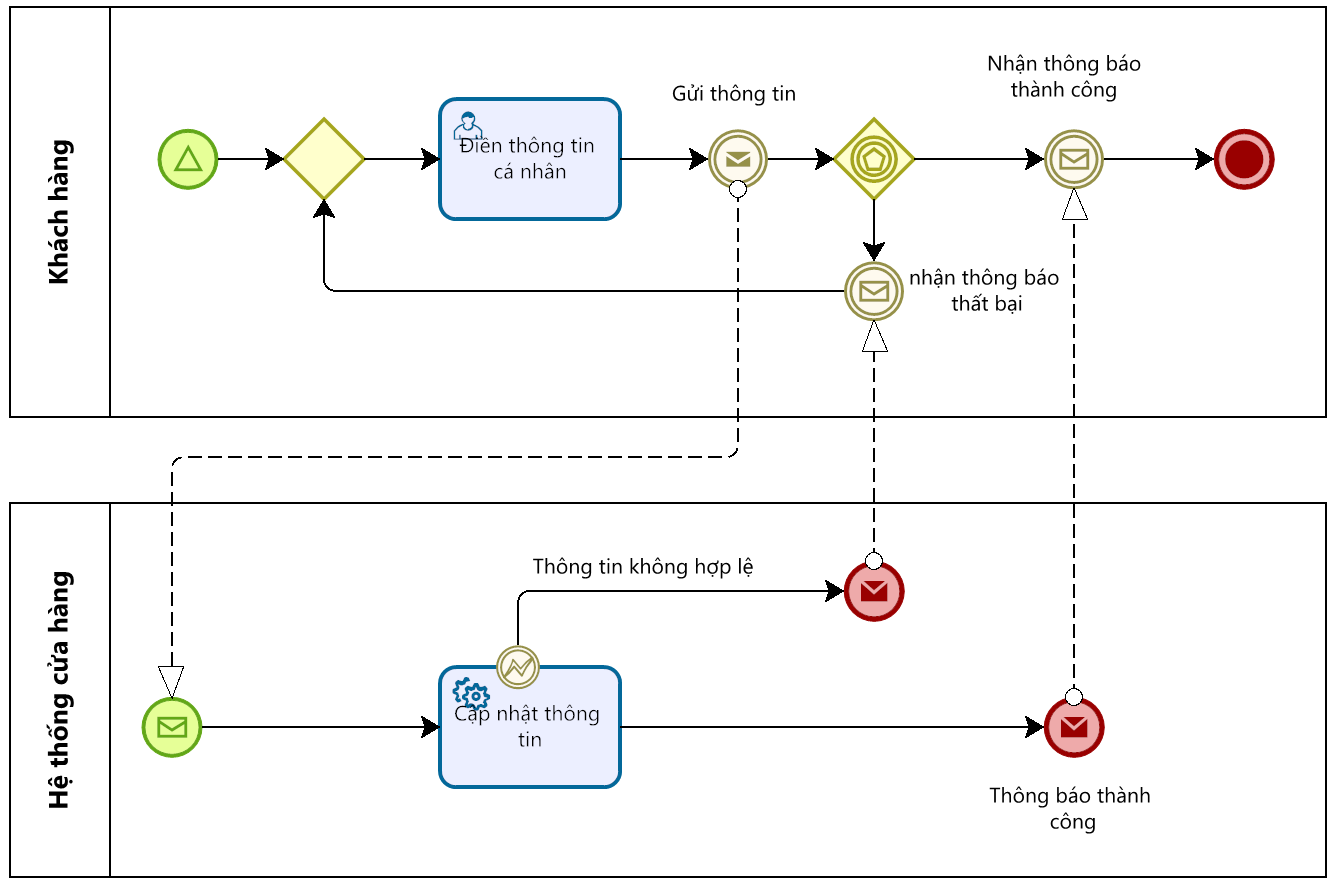
\includegraphics[width=14cm]{img/BPMN/Hien/Customer_register.png}
    \newline
    \caption{Lược đồ BPMN cho quy trình đăng ký tài khoản mới}
\end{figure}


\subsection{Làm mới mật khẩu}
\begin{figure}[!htp]
    \centering
    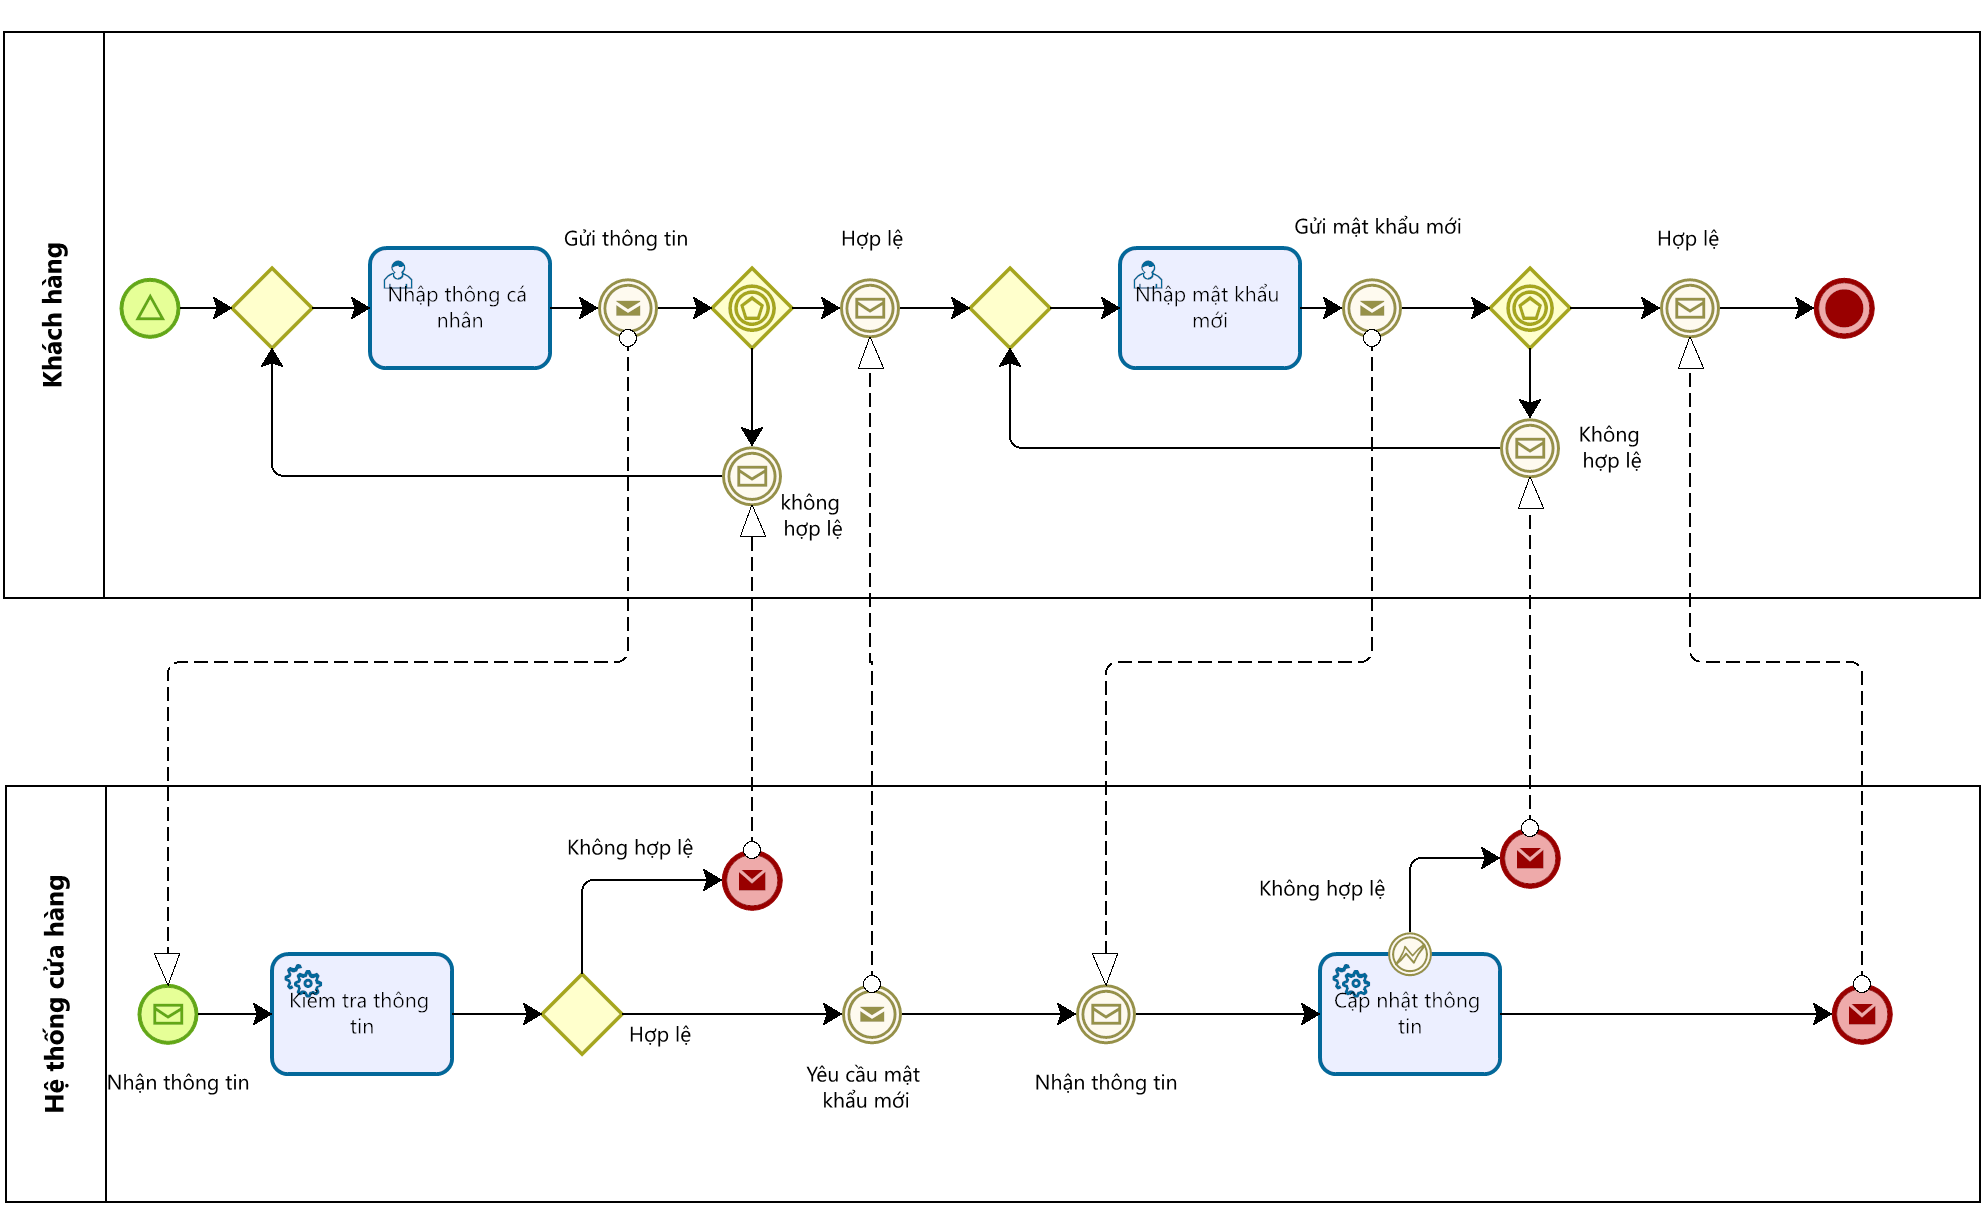
\includegraphics[width=14cm]{img/BPMN/Hien/Customer_resetPassword.png}
    \newline
    \caption{Lược đồ BPMN cho quy trình làm mới mật khẩu}
\end{figure}



\subsection{Quản lý chi nhánh}
\begin{figure}[!htp]
    \centering
    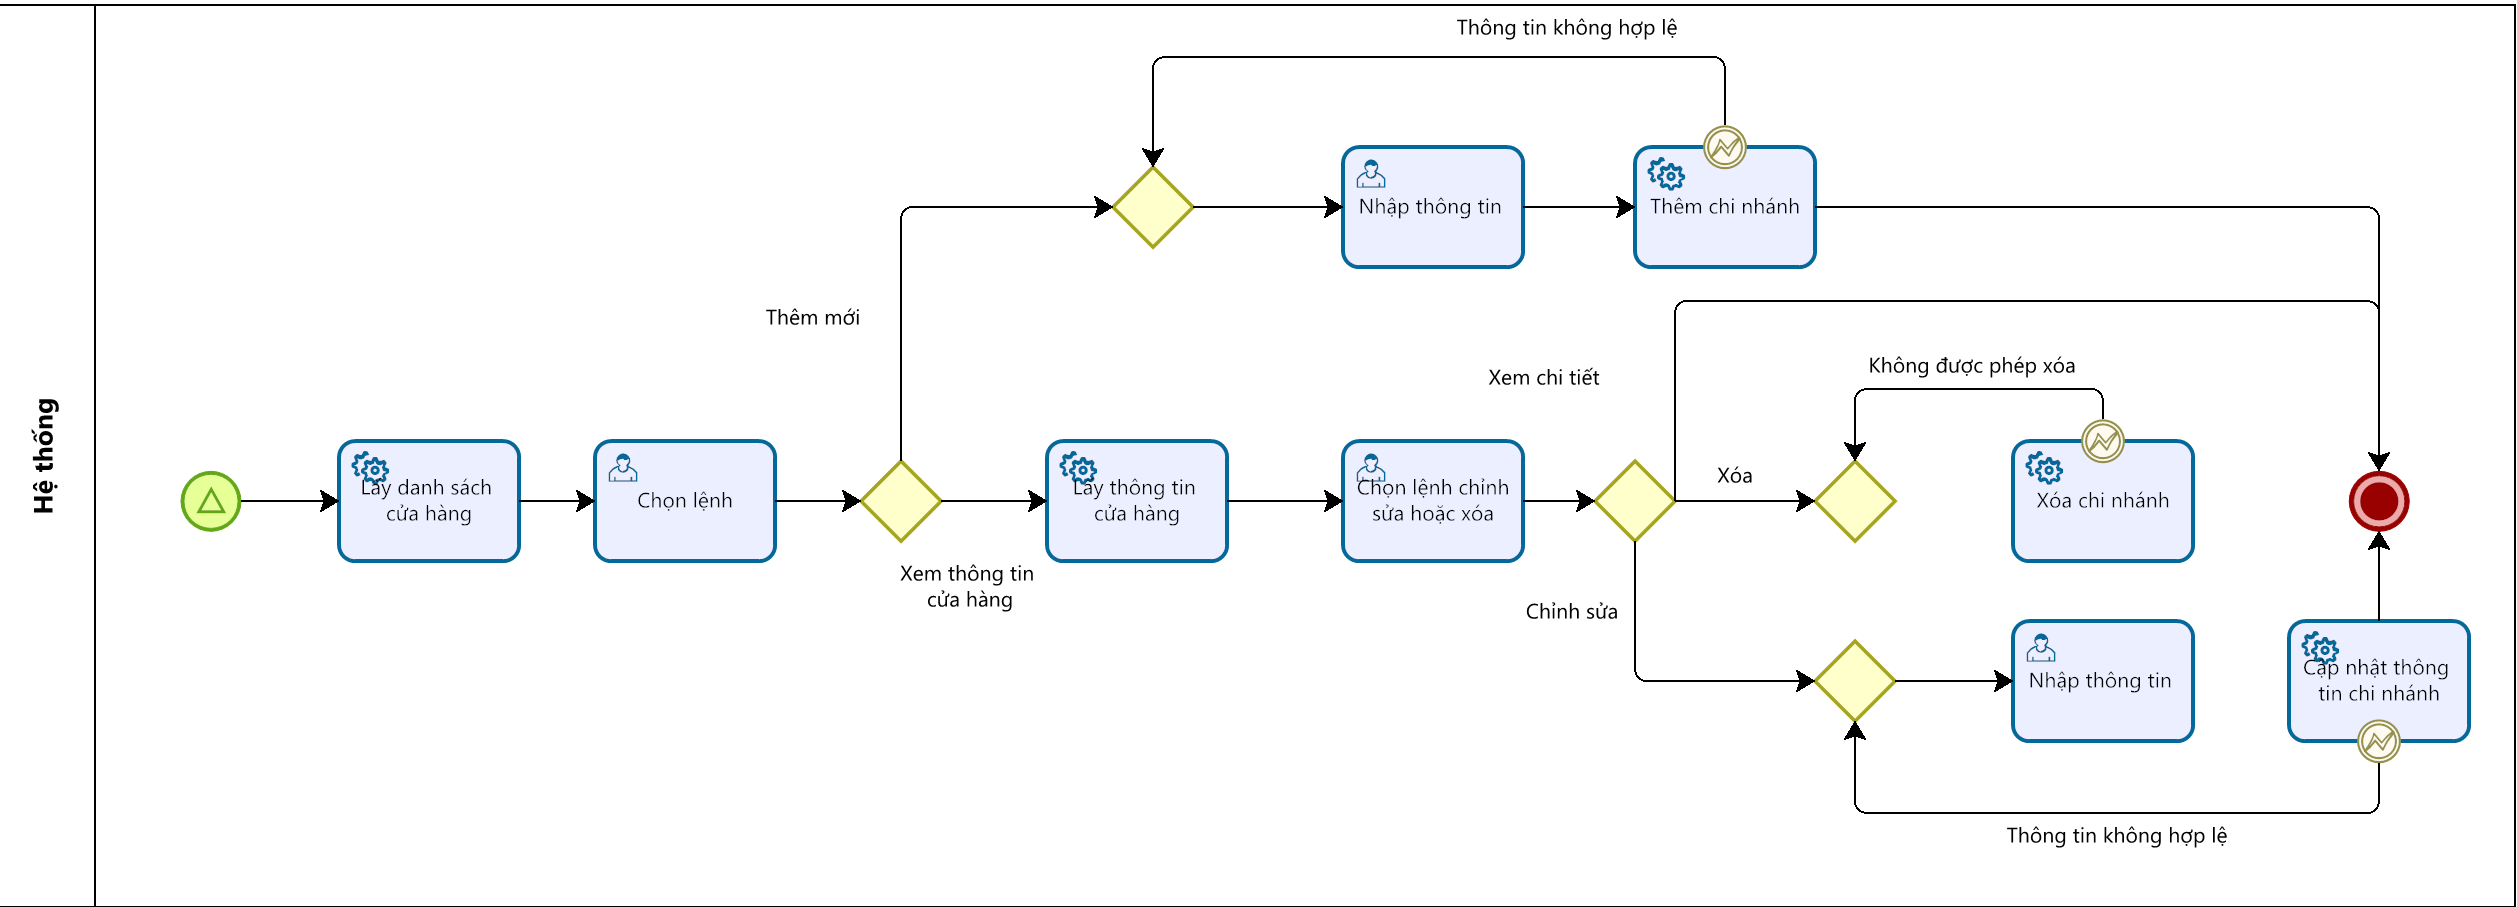
\includegraphics[width=14cm]{img/BPMN/Hien/Branch_management.png}
    \newline
    \caption{Lược đồ BPMN cho quy trình quản lý chi nhánh}
\end{figure}


\subsection{Quản lý nhân viên}
\begin{figure}[!htp]
    \centering
    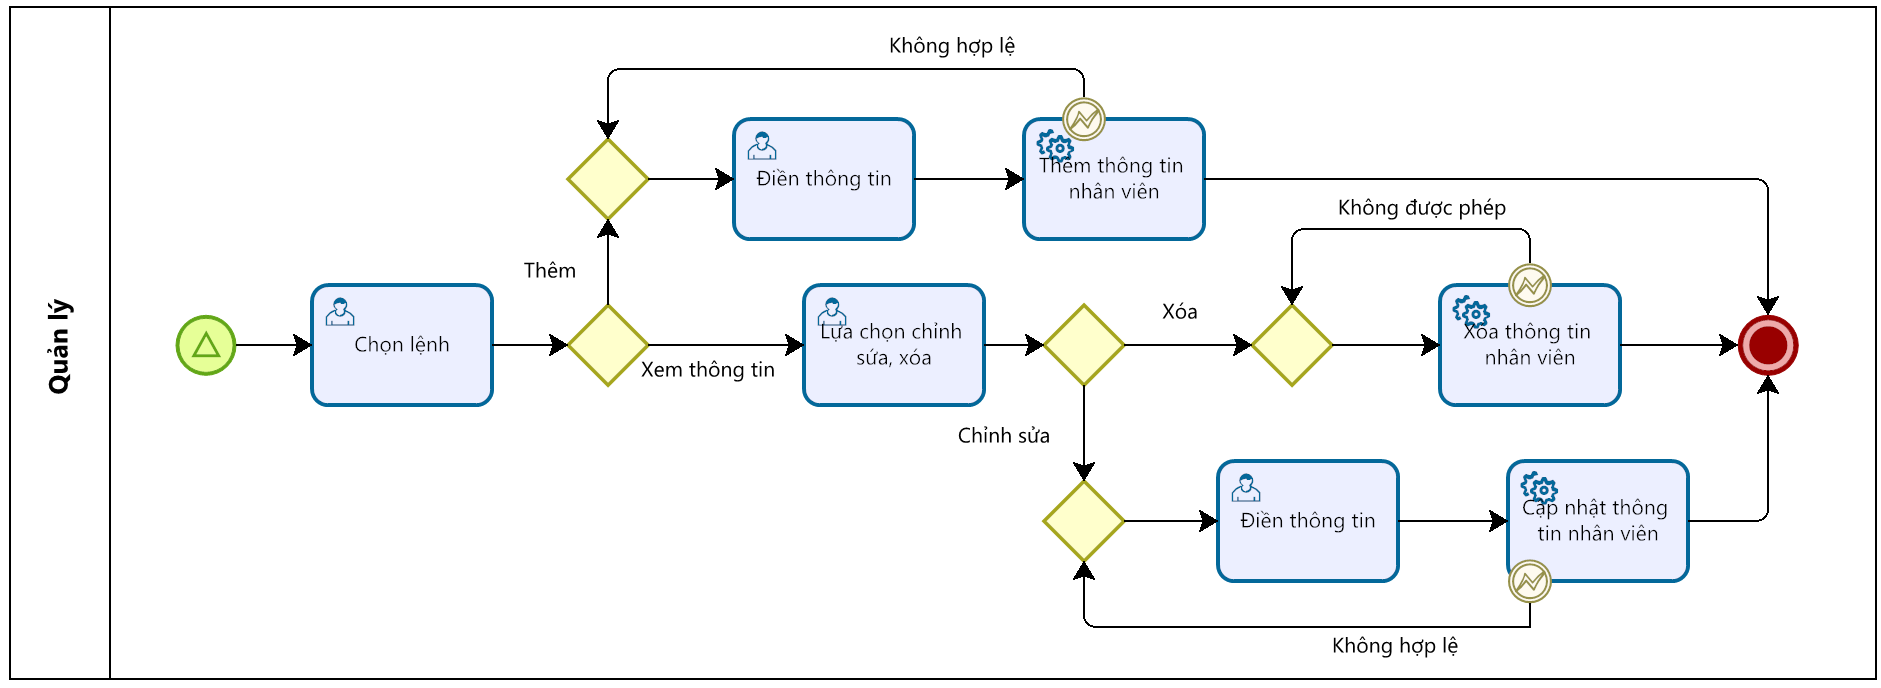
\includegraphics[width=14cm]{img/BPMN/Hien/Employee_Management.png}
    \newline
    \caption{Lược đồ BPMN cho quy trình quản lý nhân viên}
\end{figure}

\subsubsection*{Tạo yêu cầu thêm, xóa nhân viên}
\begin{figure}[!htp]
    \centering
    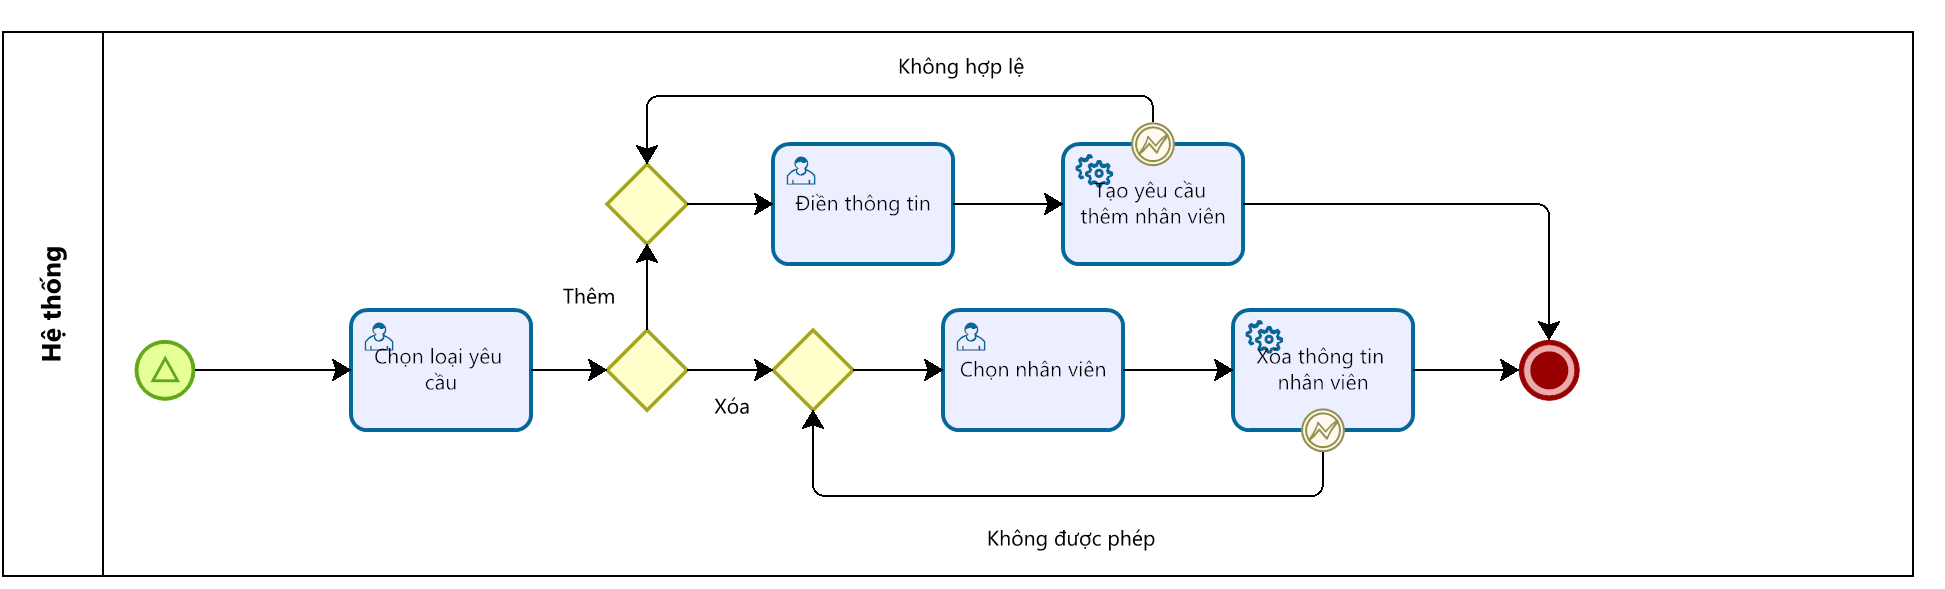
\includegraphics[width=14cm]{img/BPMN/Hien/Employee_request.png}
    \newline
    \caption{Lược đồ BPMN cho quy trình quản lý nhân viên}
\end{figure}

